%-------------------------------------------------------------------------------
% This file provides a skeleton ATLAS note.
% \pdfinclusioncopyfonts=1
% This command may be needed in order to get \ell in PDF plots to appear. Found in
% https://tex.stackexchange.com/questions/322010/pdflatex-glyph-undefined-symbols-disappear-from-included-pdf
%-------------------------------------------------------------------------------
% Specify where ATLAS LaTeX style files can be found.
\RequirePackage{latex/atlaslatexpath}
% Comment out the above line if the files are in a central location, e.g. $HOME/texmf.
%-------------------------------------------------------------------------------
\documentclass[NOTE, atlasdraft=true, texlive=2016, UKenglish]{atlasdoc}
% The language of the document must be set: usually UKenglish or USenglish.
% british and american also work!
% Commonly used options:
%  atlasdraft=true|false This document is an ATLAS draft.
%  texlive=YYYY          Specify TeX Live version (2016 is default).
%  coverpage             Create ATLAS draft cover page for collaboration circulation.
%                        See atlas-draft-cover.tex for a list of variables that should be defined.
%  cernpreprint          Create front page for a CERN preprint.
%                        See atlas-preprint-cover.tex for a list of variables that should be defined.
%  NOTE                  The document is an ATLAS note (draft).
%  PAPER                 The document is an ATLAS paper (draft).
%  CONF                  The document is a CONF note (draft).
%  PUB                   The document is a PUB note (draft).
%  BOOK                  The document is of book form, like an LOI or TDR (draft).
%  txfonts=true|false    Use txfonts rather than the default newtx.
%  paper=a4|letter       Set paper size to A4 (default) or letter.

%-------------------------------------------------------------------------------
% Extra packages:
\usepackage{atlaspackage}
% Commonly used options:
%  biblatex=true|false   Use biblatex (default) or bibtex for the bibliography.
%  backend=bibtex        Use the bibtex backend rather than biber.
%  subfigure|subfig|subcaption  to use one of these packages for figures in figures.
%  minimal               Minimal set of packages.
%  default               Standard set of packages.
%  full                  Full set of packages.
%-------------------------------------------------------------------------------
% Style file with biblatex options for ATLAS documents.
\usepackage{atlasbiblatex}
% Commonly used options:
%  backref=true|false    Turn on or off back references in the bibliography.

% Package for creating list of authors and contributors to the analysis.
\usepackage{atlascontribute}

% Useful macros
\usepackage{atlasphysics}
% See doc/atlas_physics.pdf for a list of the defined symbols.
% Default options are:
%   true:  journal, misc, particle, unit, xref
%   false: BSM, heppparticle, hepprocess, hion, jetetmiss, math, process,
%          other, snippets, texmf
% See the package for details on the options.

% Macro to add to-do notes (for several authors). Uses the todonotes package.
% \ATLnote{JS}{Jane}{green!20}{green!50!black!60}
% add macros \JSnote and \JSinote for notes in the margin and inline.
% Set output=false in order not to print out the notes.
% Comment this out for the final version of the note.
\usepackage[output=true]{atlastodo}

% Files with references for use with biblatex.
% Note that biber gives an error if it finds empty bib files.
%\addbibresource{ANA-BPHY-2019-16-INT1.bib}
\addbibresource{bib/ATLAS.bib}
\addbibresource{bib/CMS.bib}
\addbibresource{bib/ConfNotes.bib}
\addbibresource{bib/PubNotes.bib}

% Paths for figures - do not forget the / at the end of the directory name.
\graphicspath{{logos/}{figures/}}

% Add your own definitions here (file atlas-document-defs.sty).
\usepackage{ANA-BPHY-2019-16-INT1-defs}

%-------------------------------------------------------------------------------
% Generic document information.
%-------------------------------------------------------------------------------

% Title, abstract and document.
%-------------------------------------------------------------------------------
% This file contains the title, author and abstract.
% It also contains all relevant document numbers used for an ATLAS note.
%-------------------------------------------------------------------------------

% Title
\AtlasTitle{$R(K^*)$ measurement in $B_d^0 \rightarrow K^* ee/\mu\mu$}

% Draft version:
% Should be 1.0 for the first circulation, and 2.0 for the second circulation.
% If given, adds draft version on front page, a 'DRAFT' box on top of each other page, 
% and line numbers.
% Comment or remove in final version.
\AtlasVersion{0.1}

% Abstract - % directly after { is important for correct indentation.
\AtlasAbstract{%
  This note summarizes a measurement of the lepton flavour universality
  using the ratio of the branching fractions of the $B_d^0 \rightarrow K^* e^+e^-$
  and $B_d^0 \rightarrow K^* \mu^+\mu^-$, $R(K^*)$, in LHC $pp$ collision
  data recorded by the ATLAS detector at $\sqrt{s}=13$~TeV in 2018.
}

% Author - this does not work with revtex (add it after \begin{document})
%\author{The ATLAS Collaboration}

% Authors and list of contributors to the analysis.
% \AtlasAuthorContributor also adds the name to the author list.
% Include package latex/atlascontribute to use this.
% Use authblk package if there are multiple authors, which is included by latex/atlascontribute.
% \usepackage{authblk}
% Use the following 3 lines to have all institutes on one line.
% \makeatletter
% \renewcommand\AB@affilsepx{, \protect\Affilfont}
% \makeatother
% \renewcommand\Authands{, } % avoid ``. and'' for last author
% \renewcommand\Affilfont{\itshape\small} % affiliation formatting
% \AtlasAuthorContributor{First AtlasAuthorContributor}{a}{Author's contribution.}
% \AtlasAuthorContributor{Second AtlasAuthorContributor}{b}{Author's contribution.}
% \AtlasAuthorContributor{Third AtlasAuthorContributor}{a}{Author's contribution.}
% \AtlasContributor{Fourth AtlasContributor}{Contribution to the analysis.}
% \author[a]{First Author}
% \author[a]{Second Author}
% \author[b]{Third Author}
% \affil[a]{One Institution}
% \affil[b]{Another Institution}

\AtlasAuthorContributor{Biros, Marek}{a}{$\mu\mu$ data preparation (ntuple)}
\AtlasAuthorContributor{Bona, Marcella}{b}{General analysis strategies; mass fits; supervision of Nathan Heatley}
\AtlasAuthorContributor{Heatley, Nathan}{b}{Selection studies; mass fits}
\AtlasAuthorContributor{Hod, Noam}{c}{General analysis strategies; BeeX trigger efficiency studies; ML analysis; supervision of Dvij Mankad}
\AtlasAuthorContributor{Igonkina, Olga}{d}{Former analysis contact; BeeX trigger development and studies; MC preparation}
\AtlasAuthorContributor{Jakoubek, Tomas}{c}{Analysis contact; analysis framework;
  $ee$ data preparation (DAOD, ntuple), derivation update; ML analysis; fit code}
\AtlasAuthorContributor{Mankad, Dvij Chaitanya}{c}{BeeX trigger efficiency studies; ML analysis}
\AtlasAuthorContributor{Perrevoort, Ann-Kathrin}{d}{Analysis contact; consultancy for neural network,
  and general analysis strategies; MC preparation; analysis framework; $ee$ data preparation (ntuple)}
\AtlasAuthorContributor{Reznicek, Pavel}{a}{$\mu\mu$ data preparation (DAOD, ntuple); supervision of Marek Biros}
\AtlasAuthorContributor{Russell, Heather Lynn}{e}{Former analysis contact; BeeX trigger development and studies;
  $ee$ derivation development and b-phys vertexing for electrons; L1 trigger studies; MC preparation}
\AtlasAuthorContributor{Saha, Shreya}{f}{BeeX trigger development and studies; $ee$ derivation
  development and b-phys vertexing for electrons}
\AtlasAuthorContributor{Sinetckii, Viktor}{g}{$\mu\mu$ data preparation (DAOD)}
%\AtlasAuthorContributor{Walder, James}{h}{Consultancy for general analysis strategies} 
\affil[a]{Charles University, Faculty of Mathematics and Physics, Prague}
\affil[b]{Queen Mary University of London}
\affil[c]{Department of Particle Physics and Astrophysics, The Weizmann Institute of Science}
\affil[d]{FOM - Institute SAF Nikhef and University of Amsterdam/Nikhef}
\affil[e]{European Laboratory for Particle Physics, CERN}
\affil[f]{McGill University, Department of Physics}
\affil[g]{M.V.Lomonosov Moscow State University}
%\affil[h]{Rutherford Appleton Laboratory}



% If a special author list should be indicated via a link use the following code:
% Include the two lines below if you do not use atlasstyle:
% \usepackage[marginal,hang]{footmisc}
% \setlength{\footnotemargin}{0.5em}
% Use the following lines in all cases:
% \usepackage{authblk}
% \author{The ATLAS Collaboration%
% \thanks{The full author list can be found at:\newline
%   \url{https://atlas.web.cern.ch/Atlas/PUBNOTES/ATL-PHYS-PUB-2021-XXX/authorlist.pdf}}
% }

% ATLAS reference code, to help ATLAS members to locate the paper.
\AtlasRefCode{BPHY-2019-16}

% ATLAS note number. Can be an COM, INT, PUB or CONF note.
\AtlasNote{ANA-BPHY-2019-16-INT1}
% \AtlasNote{ATLAS-CONF-2021-XXX}
% \AtlasNote{ATL-PHYS-PUB-2021-XXX}
% \AtlasNote{ATL-COM-PHYS-2021-XXX}

% Author and title for the PDF file.
\hypersetup{pdftitle={ATLAS document},pdfauthor={The ATLAS Collaboration}}

%-------------------------------------------------------------------------------
% Content
%-------------------------------------------------------------------------------
\begin{document}

\maketitle

\tableofcontents

% List of contributors - print here or after the Bibliography.
% \PrintAtlasContribute{0.30}
% \clearpage

% List of to-do notes.
% \listoftodos

%-------------------------------------------------------------------------------
\section{Introduction}
\label{sec:intro}
%-------------------------------------------------------------------------------

Flavour-changing neutral currents (FCNC) have played a significant role
in the construction of the Standard Model of particle physics (SM).
These processes are forbidden at tree level and can proceed only via loops,
hence are rare. An important set of FCNC processes involve the transition
of a b quark to an s quark and two leptons, process mediated by
electroweak box and penguin diagrams as shown in Fig.~\ref{intro:fig:diagrams}.
If heavy new particles exist, they may contribute to FCNC decay amplitudes,
affecting the measurement of observables related to the decay under study.
Hence FCNC processes allow searches for contributions from sources of physics
beyond the SM (hereafter referred to as new physics).
These decays can also be exploited to test Lepton Flavour Universality
(LFU): in the SM the electroweak gauge bosons $Z$ and $W^{\pm}$ have
identical couplings to all three lepton flavours. Hence the branching
fractions of decays involving different lepton families do not depend
on the lepton flavour, but only on phase space and helicity considerations.
Any experimental evidence of violation of LFU would be a clear sign
of physics beyond the SM (BSM).

\begin{figure}[h]
\begin{center}
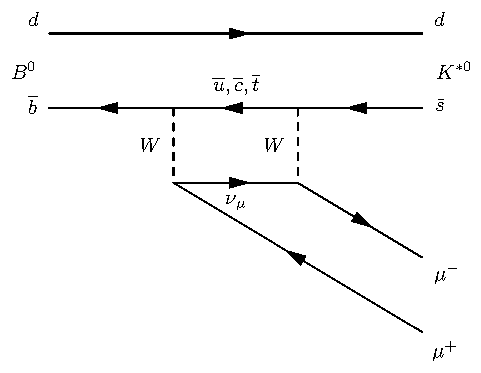
\includegraphics[width=0.45\textwidth]{figures/Feynman_diagrams-box.pdf}
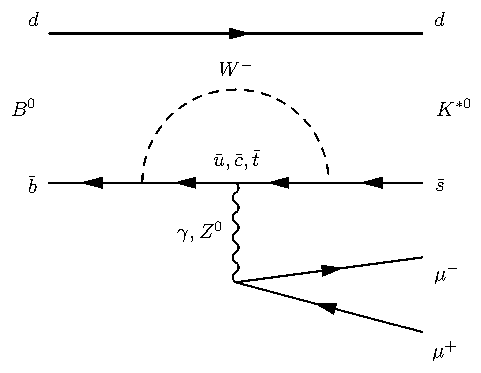
\includegraphics[width=0.45\textwidth]{figures/Feynman_diagrams-penguin.pdf}
\caption{Box and penguin Feynman diagrams of \bkstmumu decay.}
\label{intro:fig:diagrams}
\end{center}
\end{figure}

In the SM, the ratio of branching fractions of these decays is predicted to
be about unity, as the electron and muon masses are very small with respect
to that of the $b$ quark. The ratio can deviate from unity, when the value
of the dilepton invariant mass-squared ($q^2$) increases,
reducing the phase space available to the two final-state leptons.
Hence, in general the ratio is defined over a $q^2$ range $[q^2_{\mathrm min}, q^{2}_{\mathrm max}]$ as

\begin{equation}
  \label{intro:eq:rq2}
  R_{\mathrm{LFU}} \equiv \dfrac{\displaystyle\int_{q^2_{\mathrm min}}^{q^2_{\mathrm max}}
  \dfrac{\mathrm{d}\BR(\bhmumu)}{\mathrm{d}\qsqr} \mathrm{d}\qsqr}
  {\displaystyle\int_{q^2_{\mathrm min}}^{q^2_{\mathrm max}} \dfrac{\mathrm{d}\BR(\bhee)}{\mathrm{d}\qsqr} \mathrm{d}\qsqr} ~.
\end{equation}

From the experimental point of view, the detection and measurement of the
two channels with the two lepton types exploit different parts of the detector,
different reconstruction techniques and different efficiencies.
Hence a double ratio can be defined where the decays of interest are compared
with the corresponding resonant decays used as reference channels:

\begin{equation}
  \label{intro:eq:doubleratio}
  \rkst = {\frac{\BR(\bkstmumu)}{\BR(\bkstjpsimumu)}} \bigg{/} {\frac{\BR(\bkstee)}{\BR(\bkstjpsiee)}} \, .
\end{equation}


%Hereafter, the K*(892)is referred to asK∗and charge conjugation is implied
%throughout, unless stated otherwise. ratio of rates of decay into dimuon and
%dielectron final states,all as a function of the invariant mass squared
%of the dilepton systemq2. All of these observable sets canbe sensitive
%to different types of new physics that allow for FCNCs
%at tree or loop level. The BaBar, Belle,CDF, CMS, and LHCb collaborations
%have published the results of studies of the angular distributions for
%B0d→K∗μ+μ−[1–8]. The LHCb Collaboration has reported a potential hint,
%at the level of3.4standarddeviations, of a deviation from SM calculations
%[3, 4] in this decay mode when using a parameterizationof the angular
%distribution designed to minimise uncertainties from hadronic form
%factors. Measurementsusing this approach were also reported by the
%Belle and CMS Collaborations [6, 8] and they are consistentwith the
%LHCb experiment’s results and with the SM calculations. This paper
%presents results followingthe methodology outlined in Ref. [3] and
%the convention adopted by the LHCb Collaboration for thedefinition
%of angular observables described in Ref. [9].


%-------------------------------------------------------------------------------
\section{Analysis Strategy}
\label{sec:strategy}
%-------------------------------------------------------------------------------

As the electron-state trigger was activated only in 2018,
the analysis uses 2018 data only in order to have access
to both the electron and muon final states on the same
dataset.
A simple preselection is put in place in both analysis
channels to reduce the amount of events entering the
sample where the machine leaning training and the
further optimisation of the analysis choices is performed.

Section~\ref{sec:data} introduces the Monte Carlo simulation
samples used and the trigger selection on the collision data.
Section~\ref{sec:preselection} illustrates the details of the
preselection including the cut flows on both simulated samples
and collision data.








%-------------------------------------------------------------------------------
\section{Simulated and Collision Data}
\label{sec:data}
%-------------------------------------------------------------------------------

This section discusses signal Monte Carlo (MC), background MC and data samples.
For completeness the correspondence between decay mode and Monte Carlo numbers
is given in Tables~\ref{tab:data:sig} and~~\ref{tab:data:bkg} for signal-like decays
and background channels, respectively.
\begin{table}[ht] 
\caption{Simulated samples for channels used as signal, reference and control decays.} 
\centering 
\rotatebox{90}{
\begin{tabular}{l l l l l l l l }
\hline\hline 
Run & decay & prod. & filter & pdg & XS * BR * & nEvents = & Sample Weight = XS * BR * \\ [0.5ex] 
number & process & xsec (nb) & eff. & (??) & * filter eff & sum weights & * genEff * lumi /nEvents  \\ [0.5ex] 
%heading 
\hline
Signal &  &  &  &  &  &  & \\
\hline
300578 & B+ -> K+ ee & 1.24E+05 & 9.15E-02 & 5.50E-07 & 6.23E-03 & 1497000 & 1.55E-01 \\
300579 & B- -> K- ee & 1.25E+05 & 9.10E-02 & 5.50E-07 & 6.24E-03 & 1497000 & 1.55E-01 \\
300580 & B+ -> K+ J/psi(ee) & 1.24E+05 & 8.60E-02 & 6.00E-05 & 6.39E-01 & "448 & 000" \\
300581 & B- -> K- J/psi(ee) & 1.25E+05 & 8.50E-02 & 6.00E-05 & 6.36E-01 & 447000 & 5.30E+01   \\
300582 & B+ -> K+ psi(2S) (ee) & 1.24E+05 & 9.98E-02 & 4.79E-06 & 5.91E-02 & 148000 & 1.49E+01 \\
300583 & B- -> K- psi(2S) (ee) & 1.24E+05 & 9.87E-02 & 4.79E-06 & 5.89E-02 & 150000 & 1.46E+01 \\
300590 & B0 -> K*0 ee & 1.24E+05 & 5.35E-02 & 6.59E-07 & 4.36E-03 & 1497500 & 1.08E-01 \\
300591 & B0bar -> anti-K*0 ee & 1.25E+05 & 5.29E-02 & 6.59E-07 & 4.34E-03 & 1497000 & 1.08E-01 \\
300592 & B0 -> K*0 J/psi(ee) & 1.24E+05 & 5.85E-02 & 5.02E-05 & 3.63E-01 & 447500 & 3.03E+01 \\
300593 & B0bar -> anti-K*0- J/psi(ee) & 1.25E+05 & 5.80E-02 & 5.02E-05 & 3.63E-01 & 449500 & 3.01E+01 \\
300594 & B0 -> K*0 psi(2S) (ee) & 1.24E+05 & 7.37E-02 & 3.03E-06 & 2.76E-02 & 150000 & 6.86E+00 \\
300595 & B0bar -> anti-K*0 psi(2S) (ee) & 1.25E+05 & 7.31E-02 & 3.03E-06 & 2.76E-02 & 150000 & 6.87E+00 \\
300706 & Bs -> phi ee & 2.74E+04 & 6.38E-02 & 4.01E-07 & 7.01E-04 & 1500000 & 1.74E-02 \\
300707 & Bsbar -> phi ee & 2.75E+04 & 6.39E-02 & 4.01E-07 & 7.06E-04 & 1497000 & 1.76E-02 \\
300708 & Bs -> phi J/psi(ee) & 2.74E+04 & 6.71E-02 & 3.14E-05 & 5.77E-02 & 450000 & 4.78E+00 \\
300709 & Bsbar -> phi J/psi(ee) & 2.75E+04 & 6.74E-02 & 3.14E-05 & 5.82E-02 & 450000 & 4.82E+00 \\
300710 & Bs ->phi psi(2S) (ee) & 2.74E+04 & 8.74E-02 & 2.04E-06 & 4.89E-03 & 150000 & 1.22E+00 \\
300711 & Bsbar -> phi psi(2S) (ee) & 2.75E+04 & 8.82E-02 & 2.04E-06 & 4.95E-03 & 150000 & 1.23E+00 \\ 
\hline
\end{tabular} 
}
\label{tab:data:sig}
\end{table}


\begin{table}[ht] 
\caption{Simulated samples for background decay channels.} 
\centering 
\rotatebox{90}{
\begin{tabular}{l l l l l l l l } 
\hline\hline
Run & decay & prod. & filter & pdg & XS * BR * & nEvents = & Sample Weight = XS * BR * \\ [0.5ex] 
number & process & xsec (nb) & eff. & (??) & * filter eff & sum weights & * genEff * lumi /nEvents  \\ [0.5ex] 
%heading 
\hline
Background samples &  &  &  &  &  &  & \\
\hline
300718 & B+ -> pi+ J/psi(ee) & 1.24E+05 & 8.87E-02 & 2.30E-06 & 2.53E-02 & 100000 & 9.44E+00 \\
300719 & B- -> pi- J/psi(ee) & 1.25E+05 & 8.78E-02 & 2.30E-06 & 2.52E-02 & 100000 & 9.38E+00 \\
300722 & B+ -> K+ pi0(eeg) & 1.24E+05 & 1.24E-02 & 1.51E-07 & 2.32E-04 & 99000 & 8.74E-02 \\
300723 & B- -> K- pi0(eeg) & 1.25E+05 & 1.22E-02 & 1.51E-07 & 2.29E-04 & 100000 & 8.53E-02 \\
300724 & B+ -> pi+ pi0(eeg) & 1.24E+05 & 1.28E-02 & 6.46E-08 & 1.02E-04 & 99000 & 3.86E-02 \\
300725 & B- -> pi- pi0(eeg) & 1.25E+05 & 1.25E-02 & 6.46E-08 & 1.01E-04 & 100000 & 3.75E-02 \\
300726 & B+ -> pi+ eta(eeg) & 1.24E+05 & 2.29E-02 & 2.81E-08 & 7.97E-05 & "99 & 000" \\
300727 & B- -> pi- eta(eeg) & 1.24E+05 & 2.24E-02 & 2.81E-08 & 7.84E-05 & 100000 & 2.92E-02 \\
300730 & B+ -> K+ eta(eeg) & 1.24E+05 & 2.21E-02 & 1.68E-08 & 4.58E-05 & 100000 & 1.71E-02 \\
300731 & B- -> K- eta(eeg) & 1.25E+05 & 2.18E-02 & 1.68E-08 & 4.56E-05 & 100000 & 1.70E-02 \\
300734 & B0 -> K+pi- J/psi(ee) & 1.24E+05 & 5.33E-02 & 6.83E-05 & 4.50E-01 & 100000 & 1.68E+02 \\
300735 & B0bar -> K-pi+ J/psi(ee) & 1.25E+05 & 5.27E-02 & 6.83E-05 & 4.48E-01 & 100000 & 1.67E+02 \\
300738 & B0 -> K+pi- psi(2S)(ee) & 1.24E+05 & 7.31E-02 & 4.48E-06 & 4.05E-02 & 98000 & 1.54E+01 \\
300739 & B0bar -> K-pi+ psi(2S)(ee) & 1.24E+05 & 7.28E-02 & 4.48E-06 & 4.06E-02 & 100000 & 1.51E+01 \\
300742 & B0 -> K+pi- pi0(eeg) & 1.24E+05 & 4.16E-03 & 4.44E-07 & 2.28E-04 & 100000 & 8.51E-02 \\
300743 & B0bar -> K-pi+ pi0(eeg) & 1.25E+05 & 4.01E-03 & 4.44E-07 & 2.22E-04 & 100000 & 8.27E-02 \\
300744 & B0 -> K*0 eta(eeg) & 1.24E+05 & 1.53E-02 & 7.41E-08 & 1.41E-04 & 100000 & 5.24E-02 \\
300745 & B0bar -> anti-K*0- eta(eeg) & 1.25E+05 & 1.51E-02 & 7.41E-08 & 1.40E-04 & 100000 & 5.21E-02 \\
300748 & B0 -> K*0 pi0(eeg) & 1.24E+05 & 8.82E-03 & 2.58E-08 & 2.82E-05 & 100000 & 1.05E-02 \\
300749 & B0bar -> anti-K*0- pi0(eeg) & 1.24E+05 & 8.65E-03 & 2.58E-08 & 2.78E-05 & 100000 & 1.04E-02 \\
\hline
\end{tabular} 
}
\label{tab:data:bkg}
\end{table}




We define the following decay labels:
\begin{itemize}
\setlength{\itemsep}{0pt}%
\setlength{\parskip}{0pt}%
  \item signal channel (or non-resonant signal channel): $B^\pm \to K^{*0}\ell\ell$;
  \item reference channel (or resonant signal channel): $B^\pm \to K^{*0}J/\psi(\ell\ell)$;
  \item control channel: $B^\pm \to K^{*0}\psi(2S)(\ell\ell)$;
\end{itemize}

We then consider all the other modes in Tables~\ref{tab:data:sig} and~~\ref{tab:data:bkg}
as possible B backgrounds when reconstructed in the final state of two leptons and two mesons.







%-------------------------------------------------------------------------------
\section{Trigger Selections}
\label{sec:trigger}
%-------------------------------------------------------------------------------
\subsection{Trigger for the electron final states}
\label{subsec:trigger-for-electron}

The trigger used for the selection of the electron final state are mainly
described in Sec.~4.2.5 in~\ref{ATL-DAQ-PUB-2019-001}.

[Text and plots from ATL-DAQ-PUB-2019-001 to have a starting point]\\
In 2018, a new set of triggers was added to select low-\pT dielectron events within an
invariant mass region corresponding to decays of $b$-hadrons. The development focused on
$B^{0}\rightarrow K^{*} e^{+}e^{-}$ decays, but all triggers developed are agnostic to
additional tracks, and thus are also sensitive to \emph{e.g.}
$B^{+}\rightarrow K^{+} e^{+}e^{-}$ decays.

Both L1 items and HLT algorithms were developed.
% L1_BPH-0M9-EM7-EM5
% L1_BPH-0DR3-EM7J15
Mimicking the $B$-physics L1 muon strategy, L1 topological triggers using EM RoIs were developed.
The main trigger requires the invariant mass between two L1 EM RoIs, one with $\ET > 7$~GeV (EM7)
and the second with $\ET > 5$~GeV (EM5), to be less than 9~GeV.
However, since the granularity of the L1 calorimeter trigger is somewhat coarser than the extent
of a single, low-\pT electron, when the two electrons are very close-by they will only create
a single L1 EM RoI in the detector.  Thus, a L1 trigger for close-by electrons was created,
which requires a L1 EM RoI within $\Delta R < 0.3$ of a L1 jet RoI.
These two situations are depicted in Figure~\ref{fig:BeeK_sketch}.

\begin{figure}[htbp]
  \centering %trim = 0.9cm 0 1.5cm 0, clip,
  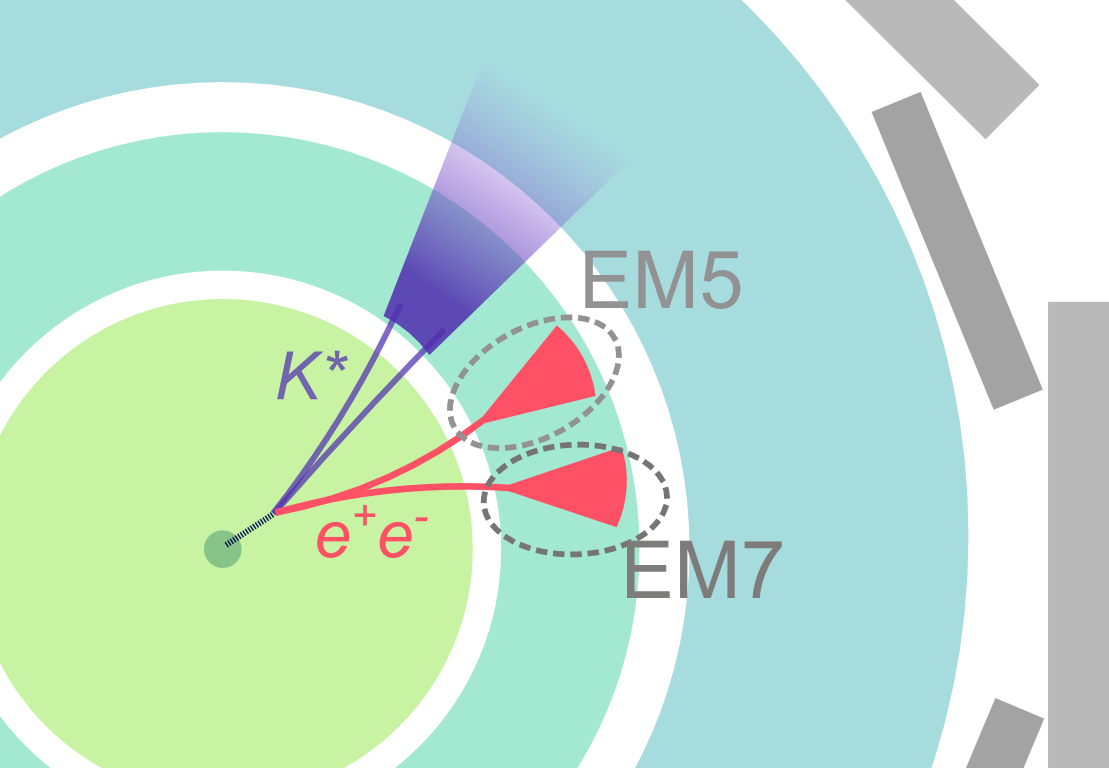
\includegraphics[width=.35\textwidth]{figures/BtoKstaree_separated}
  ~~~~~~~~~~~~
  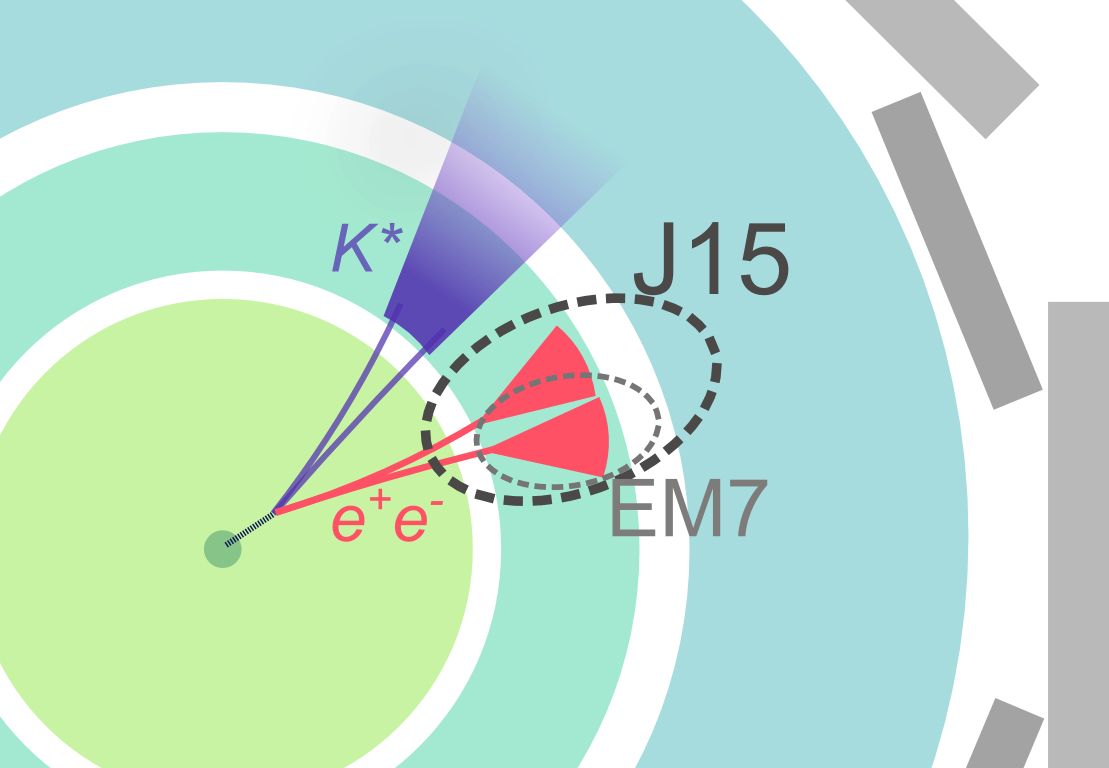
\includegraphics[width=.35\textwidth]{figures/BtoKstaree_close}
  \caption{
    Topological sketches of $B\rightarrow K^{*} e^{+}e^{-}$ decays, where, from the point of view of
    the L1 EM RoIs, the two electrons are well-separated (left), and the two electrons are overlapping
    (right). From the centre outwards, the colours represent the inner detector, electromagnetic
    calorimeter, hadronic calorimeter, and first layer of the muon spectrometer.
  }
  \label{fig:BeeK_sketch}
\end{figure}

On their own, the rates of these two L1 triggers are greater than the global 100 kHz limit,
and thus they are combined with a muon requirement to lower the rate: either one MU6 muon or
two MU4 muons. Because the production of one $b$-hadron is likely to result in the production
of another, the muon requirement provides a higher purity sample than simply prescaling
the original L1 triggers. The rates of the two L1 EM-based triggers with and without
combination with the L1 muon selections are shown in Figure~\ref{fig:BeeK_L1Rates}.

\begin{figure}[htbp]
  \centering %trim = 0.9cm 0 1.5cm 0, clip,
    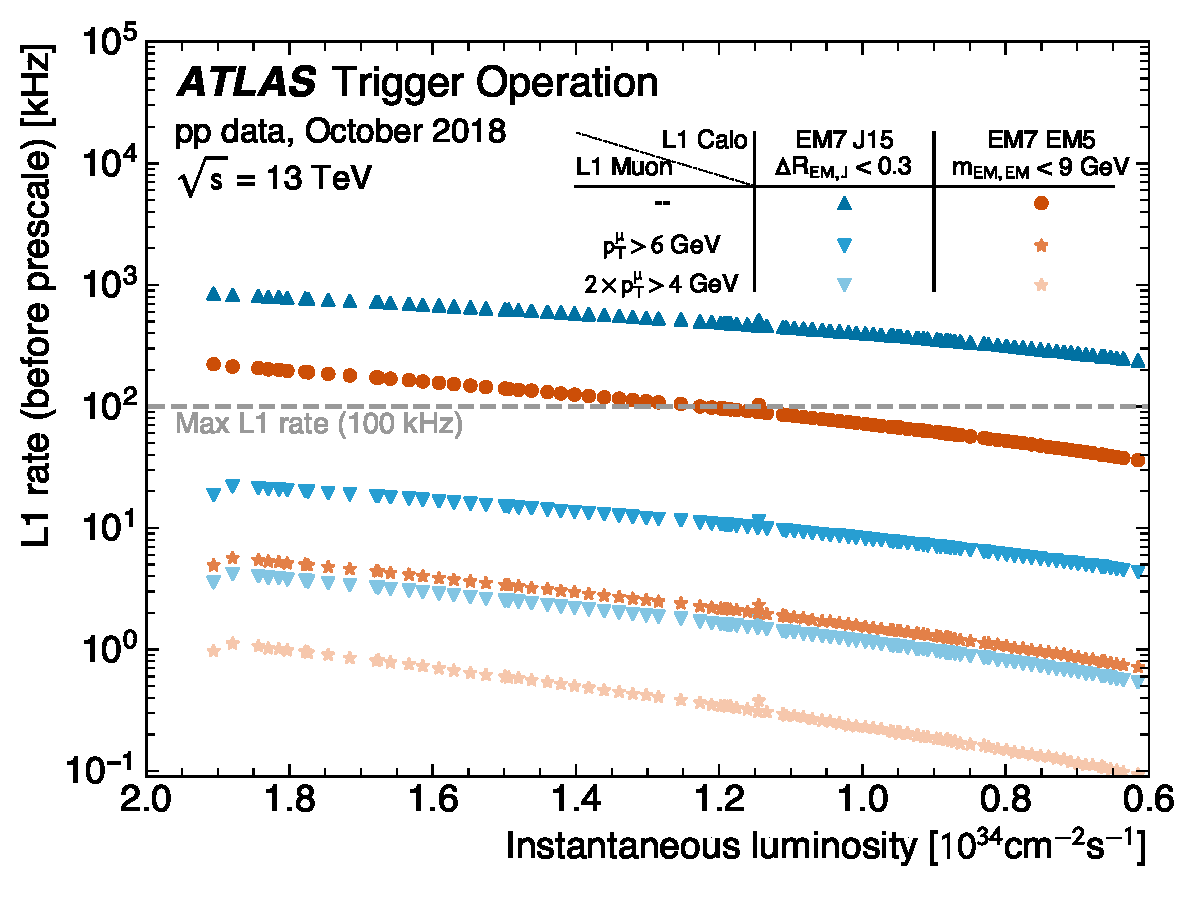
\includegraphics[width=.65\textwidth]{figures/L1BPH_rates_ATLASStyle}
  \caption{
  L1 trigger rate, before the application of any prescale, as a function of instantaneous
  luminosity for the two L1 items targeting $B\rightarrow K^{*} e^{+}e^{-}$ decays alone
  and in association with either one 6~GeV muon or two 4~GeV muons. The L1 calorimeter-based
  thresholds for an EM RoI with $\ET > 5$~GeV, an EM RoI with $\ET > 7$~GeV, and a jet RoI
  with $\ET > 15$~GeV, are represented by EM5, EM7, and J15, respectively.
  The four triggers with an L1 muon requirement were deployed online, with end-of-fill prescale strategies.
  }
  \label{fig:BeeK_L1Rates}
\end{figure}

For the L1 trigger with two L1 EM RoIs, two electrons matching the L1 EM RoIs are required
in the HLT, with $\ET^{1} >  9$~GeV and $\ET^{2} > 5$~GeV. For the single L1 EM RoI trigger,
two HLT electrons with 5~GeV are required. The HLT electrons were required to pass a very
loose electron likelihood (LH) PID~\cite{ATLAS-CONF-2016-024}, without any requirement on
the transverse impact parameter. The electrons are required to form a vertex with $\chi^2 < 20$,
and the invariant mass of the vertex must be between 0.1 and 6~GeV, which is inclusive
of all relevant $b$-hadron decays. Additionally, HLT muons are required in parallel with
the L1 muon requirement (either one 6~GeV or 2, 4~GeV HLT muons). These four triggers were
deployed on 8 June 2018. An end-of-fill strategy was applied to all triggers except the
one with 2, 4~GeV muons and electron thresholds of 9~GeV and 5~GeV, to account for the large L1 rates.

Due to the additional muon requirement, the aforementioned triggers were not fully efficient
for signal events, and thus a second set of triggers was developed without the muon requirement.
However, as demonstrated in Figure~\ref{fig:BeeK_L1Rates}, running electron-only items
at L1 was not feasible. Thus, instead of requiring dedicated L1 triggers, an HLT trigger
was instead run over every event selected by the L1 trigger (L1 accept). HLT electron
reconstruction was seeded from EM3 RoIs and two separate triggers were used, one for
well-separated electrons and one for close-by electrons. In both cases, two 5~GeV HLT electrons
passing a very loose electron LH PID, without any requirement on the transverse impact parameter,
are required, with the same vertex requirements as the seeded triggers. It should be noted that,
although this trigger ran without an HLT prescale, it only ran if there was an L1 accept
from the rest of the trigger menu. %However, the L1 accept is biased towards high-\pT physics\
 and thus provides a hard scatter-enriched environment that is more likely to contain
 signal events than any given event with low-\pT EM~RoIs. [speculation]

\begin{figure}[h!]
  \centering %trim = 0.9cm 0 1.5cm 0, clip,
  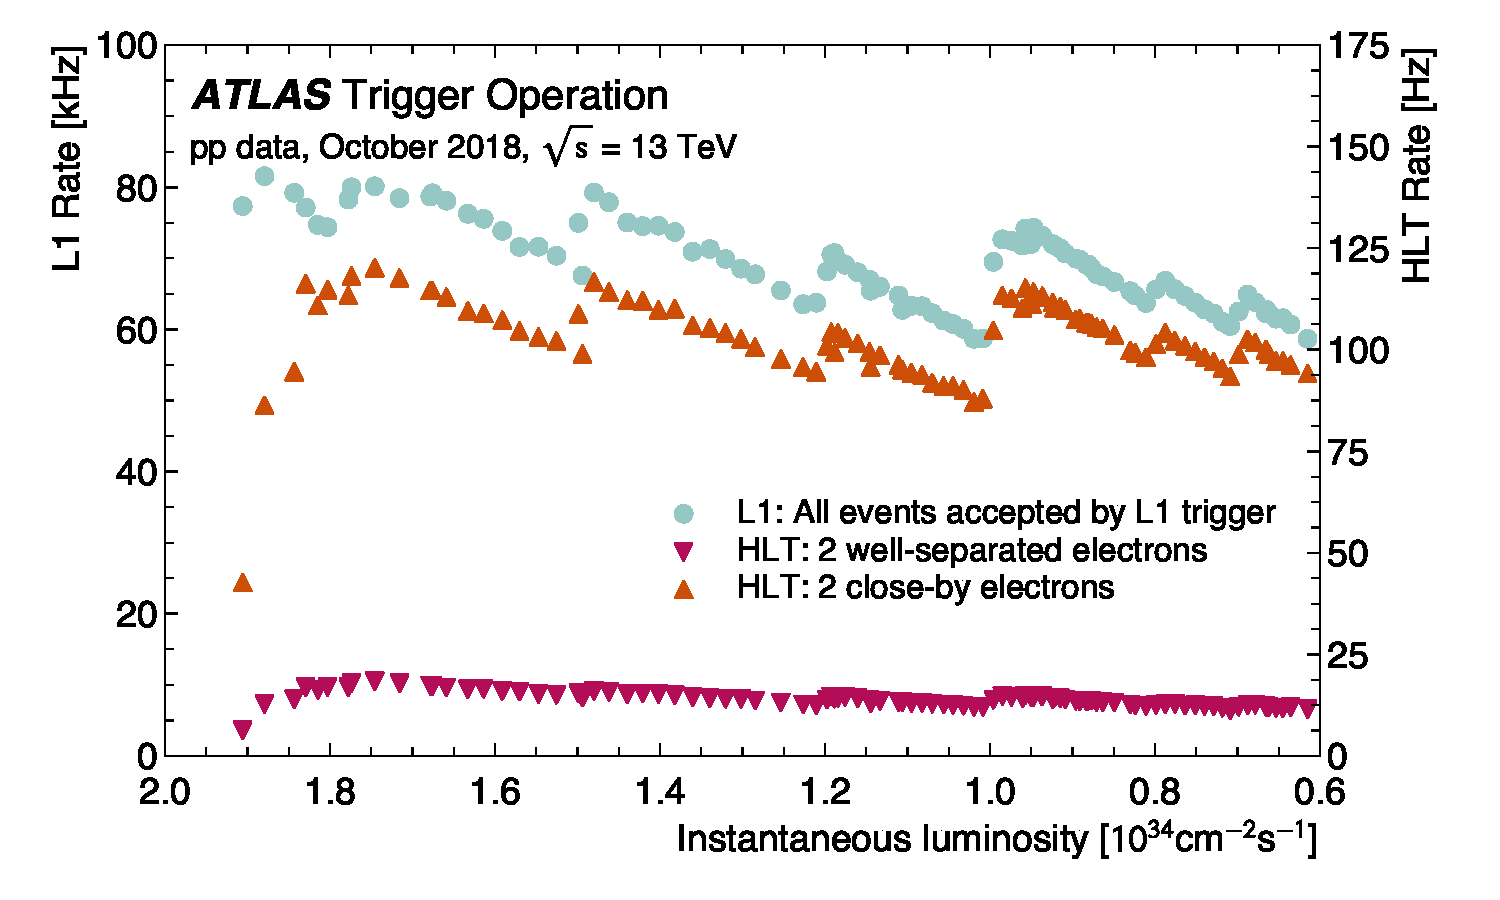
\includegraphics[width=0.65\textwidth]{figures/BeeK_OctOnly_ATLAS}
  \caption{L1 and HLT trigger rates as a function of instantaneous luminosity for the two
  unseeded triggers targeting $B\rightarrow K^{*} e^{+}e^{-}$ decays.
  }
  \label{fig:BeeK_HLT_unseeded}
\end{figure}

These unseeded triggers were deployed on 14~July~2018, and ran without any HLT prescale below
luminosities of \lumi{1.85}. Above this, small HLT prescales were applied to reduce the
excessive pressure on the readout system required to run low-\pT electron reconstruction
in every event accepted by the L1 trigger: 5 above \lumi{2}, 2.5 between \lumi{1.95} and
\lumi{2}, and 1.5 between \lumi{1.85} and \lumi{1.95}. These HLT prescales were achieved
by online adjustments until the optimal running scenario was achieved.
Figure~\ref{fig:BeeK_HLT_unseeded} shows the L1 accept rate and HLT rates of each of the
two unseeded triggers as a function of instantaneous luminosity, for a run in October 2018.

\subsection{Trigger for the muon final states}

Events with the muon final states are selected using the \texttt{HLT\_2mu6\_bBmumuxv2\_L1LFV-MU6} trigger.
The level-1 (L1) trigger identifies two regions of interest (RoI) with $p_T > 6$~GeV and opening angle $\Delta R < 1.5$.
The level-2 trigger requires a di-muon vertex with $\chi^2 < 20$ and $0.1 < m_{\mu\mu} < 6.5$~GeV,
two opposite-charged tracks fitted to a common vertex with $\chi^2 < 20$ and mass in range $0.1 - 15$~GeV.
In the Event Filter, the $B^0_d \rightarrow K^{*0} \mu^+ \mu^-$ vertex is reconstructed with  $B^0_d$-vertex $\chi^2 < 60$, $K^{*0}$-vertex $\chi^2 < 400$, $m_{B_d} \in [4.6, 5.9]$~GeV and $m_{K^{*0}} \in [0.7, 1.1]$~GeV.

The trigger efficiency, defined as the ratio of events firing the trigger to those passing the offline selections,
is a crucial part of the total efficiency. It is modelled by the MC sample in bins of $p_T$ and charge-signed pseudorapidity $q\eta$ of the two muons, $\Delta R$ and rapidity of the di-muon, and  di-meson $p_T$ of the di-tracks. The mismodelling of MC trigger efficiency can be corrected by the efficiency scale factor. The scale factor consist of two parts. The first part is obtained from the official tool for measurement of B-physics trigger efficiency scale factors. For a normal di-muon trigger, the strategy of the tool is to factorise the efficiency as 

\begin{equation}
\varepsilon_{\mu\mu} = \varepsilon(\mu_1, \mu_2 \leftrightarrow \text{muX, muY})\times c_{\mu\mu}(\Delta R, |y^{\mu\mu}|),
\end{equation}

where $\varepsilon(\mu_1, \mu_2 \leftrightarrow \text{muX, muY})$ is the efficiency for the single muon legs
to identify the RoIs of the two muons, X and Y represent the $p_T$ thresholds of the two legs,
and $c_{\mu\mu}(\Delta R, |y^{\mu\mu}|)$ is the di-muon correction accounting for the inefficiency due to di-muon effect.

Assuming $\text{Y} > \text{X}$, the first term can be further broken down as

\begin{equation}
\begin{aligned}
  &\varepsilon(\mu_1, \mu_2 \leftrightarrow \text{muX, muY}) \\
  &= \varepsilon_{\text{muY}}(1)[\varepsilon_{\text{muX}}(2)-\varepsilon_{\text{muY}}(2)]
    +\varepsilon_{\text{muY}}(2)[\varepsilon_{\text{muX}}(1)-\varepsilon_{\text{muY}}(1)]
    +\varepsilon_{\text{muY}}(1)\varepsilon_{\text{muY}}(2) \\
  &=\varepsilon_{\text{muX}}(1)\varepsilon_{\text{muY}}(2)
    +\varepsilon_{\text{muX}}(2)\varepsilon_{\text{muY}}(1)
    -\varepsilon_{\text{muY}}(1)\varepsilon_{\text{muY}}(2)
\end{aligned},
\end{equation}

where $\varepsilon_{\text{muX}}(1) \equiv \varepsilon_{\text{muX}}(p^{(1)}_T, q\eta^{(1)})$ is the single muon efficiency.
The charge-signed pseudorapidity $q\eta$ instead of normal pseudorapidity is used to account
for the charge dependence of reconstruction in the toroidal magnetic field of the muon spectrometer.
For symmetric triggers, this term simply reduces to $\varepsilon_{\text{muX}}(1)\varepsilon_{\text{muX}}(2)$.

The di-muon correction can be broken down into

\begin{equation}
c_{\mu\mu}(\Delta R, |y^{\mu\mu}|) = c_{\Delta R}(\Delta R, |y^{\mu\mu}|) \times c_a(|y^{\mu\mu}|),
\end{equation}

where $c_{\Delta R}(\Delta R, |y^{\mu\mu}|)$ is the $\Delta R$ correction accounting for the loss of
efficiency at small $\Delta R$ where the RoIs can be overlapping, and $c_a(|y^{\mu\mu}|)$
is the asymptotic correction accounting for the loss of efficiency due to the opposite charge
and vertex requirement.

The $\Delta R$ correction $c_{\Delta R}$, asymptotic correction $c_a$ and single muon efficiency $\varepsilon_{\text{muX}}$ are obtained by different methods described below using $J/\psi \rightarrow \mu^+ \mu^-$ sample. The scale factor is then computed as the ratio of the data efficiency to MC efficiency .

The second part of the scale factor handles the track selection of \texttt{HLT\_2mu6\_bBmumuxv2\_L1LFV-MU6}. The track selection efficiency is obtained from the fraction of $B^0_d \rightarrow K^{*0} J/\psi(\mu^+ \mu^-)$ candidates passing both \texttt{HLT\_2mu6\_bBmumuxv2\_L1LFV-MU6} and \texttt{HLT\_mu11\_mu6\_bDimu} among those only being required to pass \texttt{HLT\_mu11\_mu6\_bDimu}.

\subsubsection{$\Delta R$ correction}
The $\Delta R$ correction is obtained by di-muon tag-and-probe method.
The tag muon should match to HLT muon of the tag triggers with $\Delta R < 0.01$,
and match to L1 RoI by $\Delta R < \text{L1Cut}(p_T)$, where

\begin{equation}
\text{L1Cut}(p_T) = \left\{
\begin{aligned}
-0.01p_T + 0.18 &, \text{ if } p_T < 10 \text{ GeV} \\
0.08 &, \text{ otherwise}
\end{aligned}
\right.
\end{equation}

In 2017, \texttt{HLT\_mu14\_bJpsi\_TrkPEB} and \texttt{HLT\_mu20\_bJpsi\_TrkPEB} are used as tag triggers
for $c_{\Delta R}$. In 2018, only \texttt{HLT\_mu10\_bJpsi\_TrkPEB} is used as tag trigger.

To correctly extract $\Delta R$ correction, additional event selections are required:

\begin{itemize}
\item $p_T > 12 \text{ GeV}$ for both muons, to make sure $\varepsilon_{\text{muX}}$ is at the plateau to get rid of single muon effect.
\item Events un-prescaled with respect to the di-muon trigger.
\end{itemize} 

The ratio $\rho_{\Delta R}$ is defined as

\begin{equation}
\rho_{\Delta R}(\Delta R, |y^{\mu\mu}|) = \dfrac{N(\text{tagged + accepted by \texttt{HLT\_2mu10\_bJpsimumu}})}{N(\text{tagged by \texttt{HLT\_mu10\_bJpsi\_TrkPEB}})},
\end{equation}

where the number of candidates in each $(\Delta R, |y^\mu\mu|)$ bin is obtained by fitting to the di-muon invariant mass distribution.
An example is shown in Figure~\ref{fig:fit_example}.

\begin{figure}[h]
\center
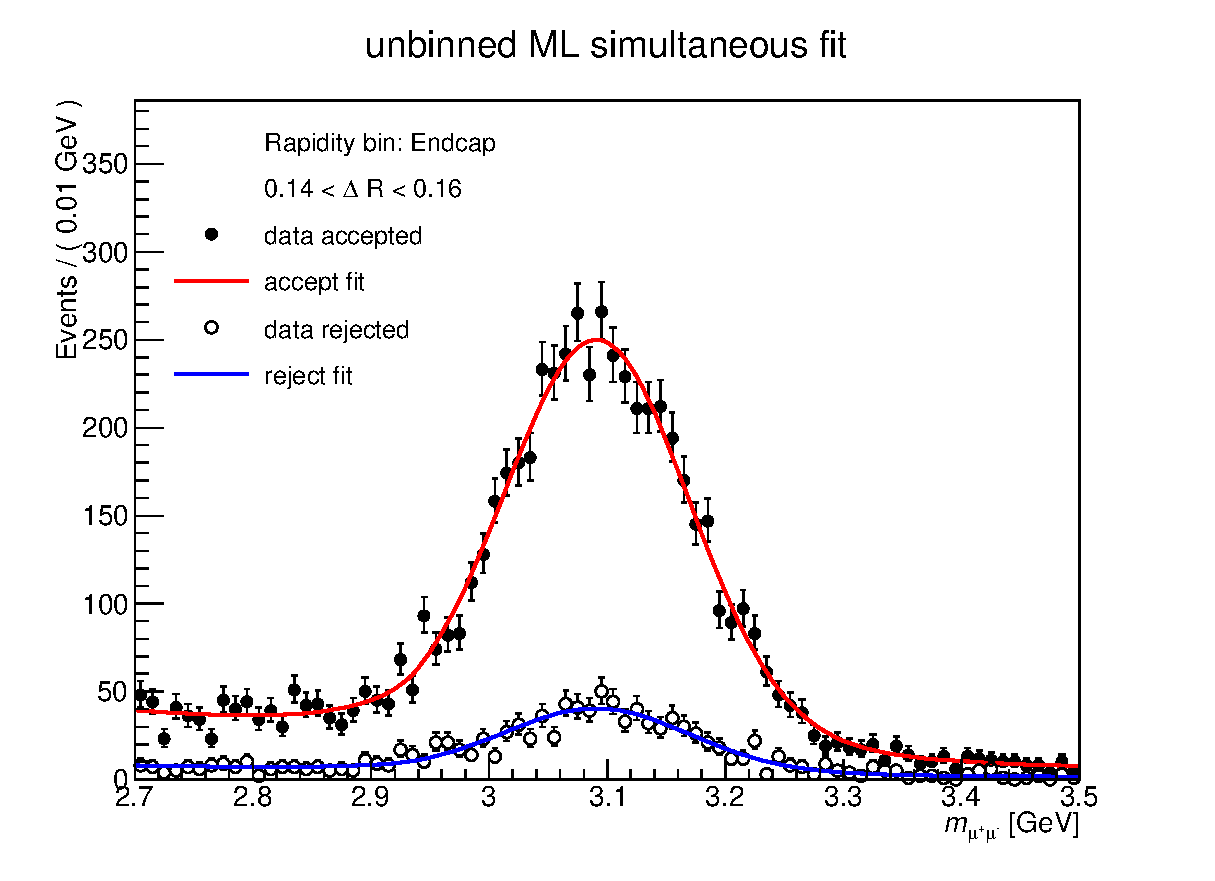
\includegraphics[width=12cm,height=8.28cm]{fit_example.eps} 
\caption{An example of the unbinned maximum likelihood fit to the di-muon invariant mass distribution
  to extract the number of candidates in the bin $0.14< \Delta R < 0.16$ and $1.2 < |y^{\mu\mu}| < 2.4$.
  The fit function consists of a Gaussian plus one-sided Crystal-Ball signal and an exponential background.
  The red (blue) curve is the fit to candidates accepted (rejected) by the di-muon trigger.}
\label{fig:fit_example}
\end{figure}

$\rho_{\Delta R}$ is fitted against $\Delta R$ with an error function with a normalization 

\begin{equation}
f(x;p_0,p_1,p_2) = p_2\text{Erf}[(x+p_0)/p_1]
\end{equation}

in three rapidity $|y^{\mu\mu}|$ regions: barrel ($0 < |y^{\mu\mu}| < 1.05$), overlap ($1.05 < |y^{\mu\mu}| < 1.2$)
and endcap ($1.2 < |y^{\mu\mu}| < 2.4$). The result of the fits are shown in Figure~\ref{fig:fit_rho_dr}.

\begin{figure}[h]
\center
\hspace{-0.1cm}
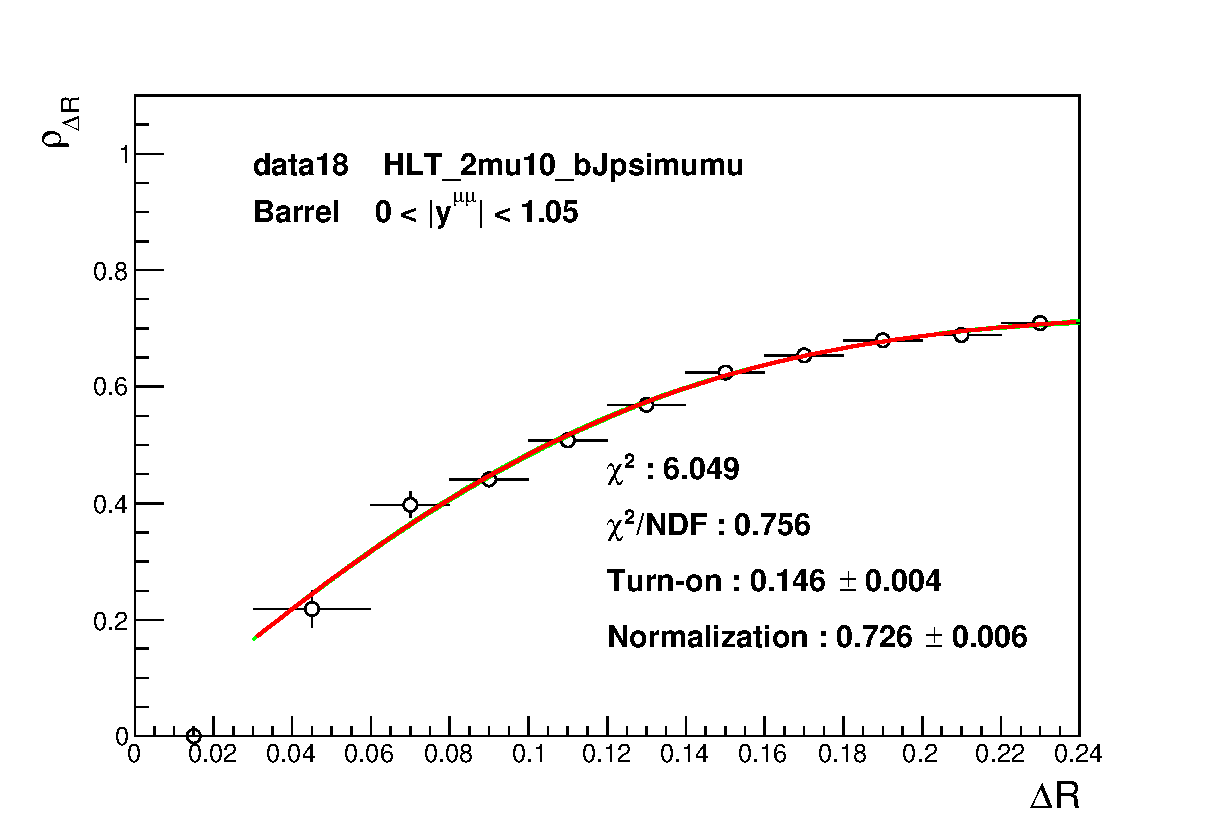
\includegraphics[width=0.33\textwidth]{htg_efficiency_Barrel_HLT_2mu10_bJpsimumu_Data18AllYear.eps} 
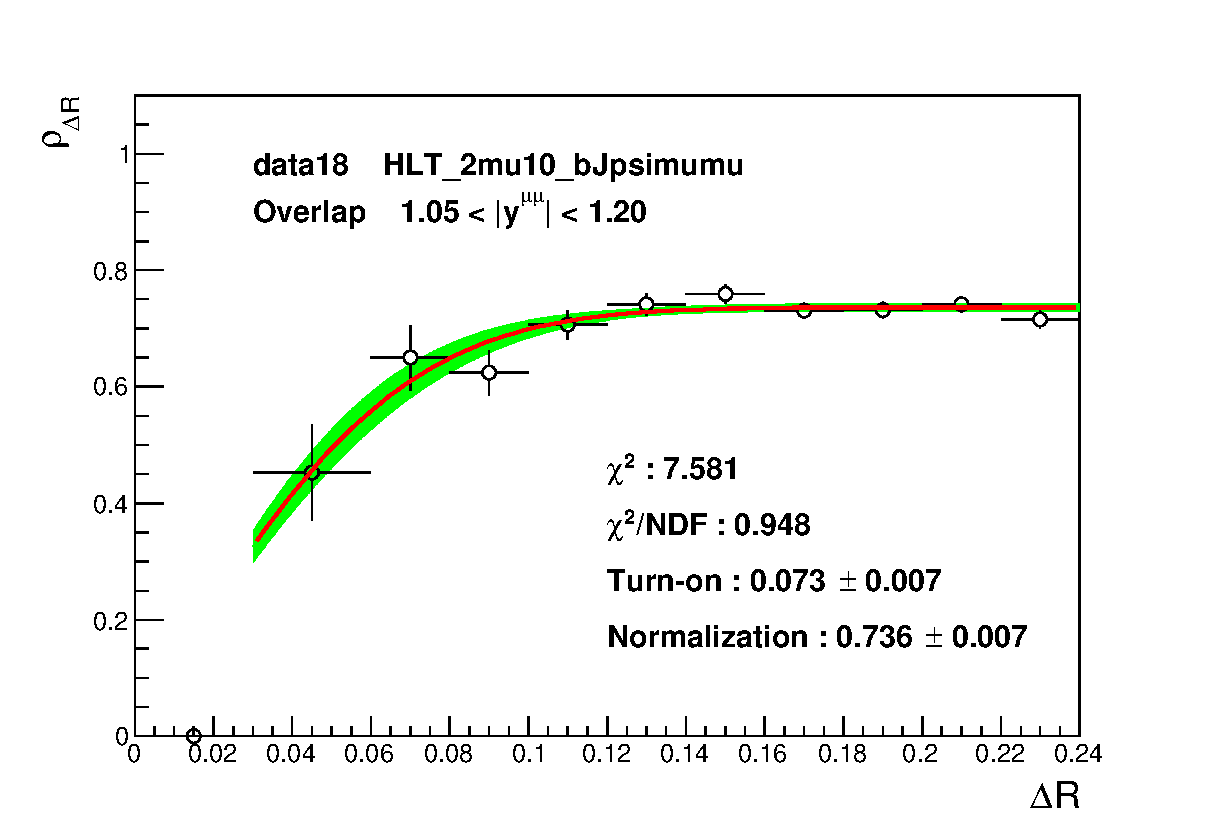
\includegraphics[width=0.33\textwidth]{htg_efficiency_Overlap_HLT_2mu10_bJpsimumu_Data18AllYear.eps} 
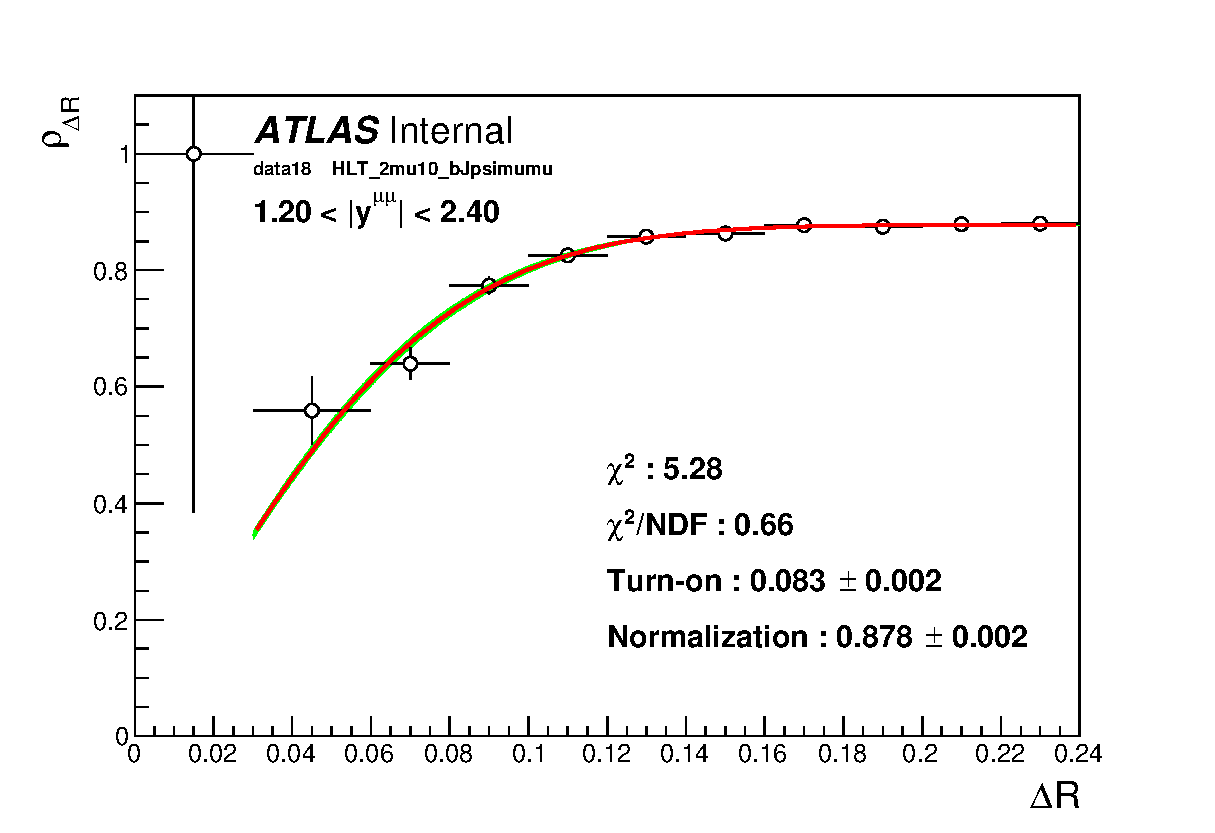
\includegraphics[width=0.33\textwidth]{htg_efficiency_Endcap_HLT_2mu10_bJpsimumu_Data18AllYear.eps} \\
\hspace{-0.1cm}
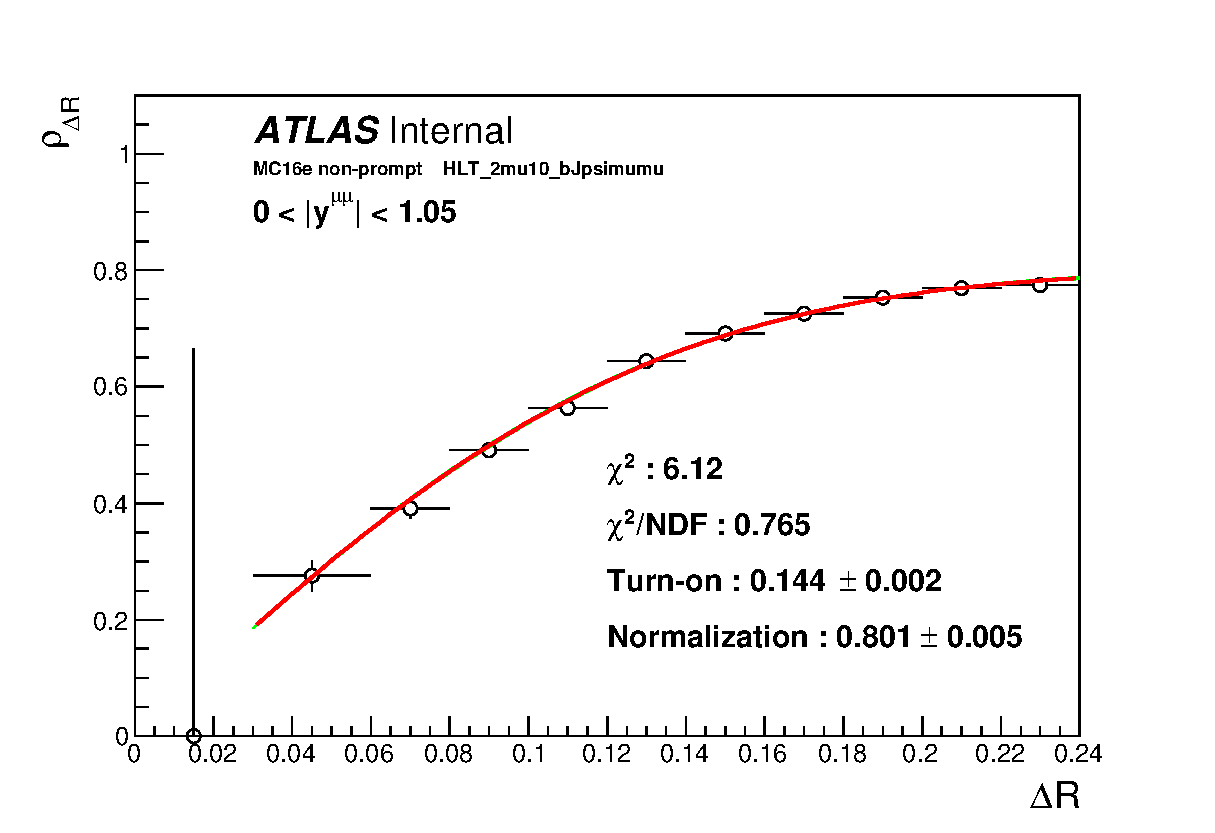
\includegraphics[width=0.33\textwidth]{htg_efficiency_Barrel_HLT_2mu10_bJpsimumu_undefined_periodMC16e.eps} 
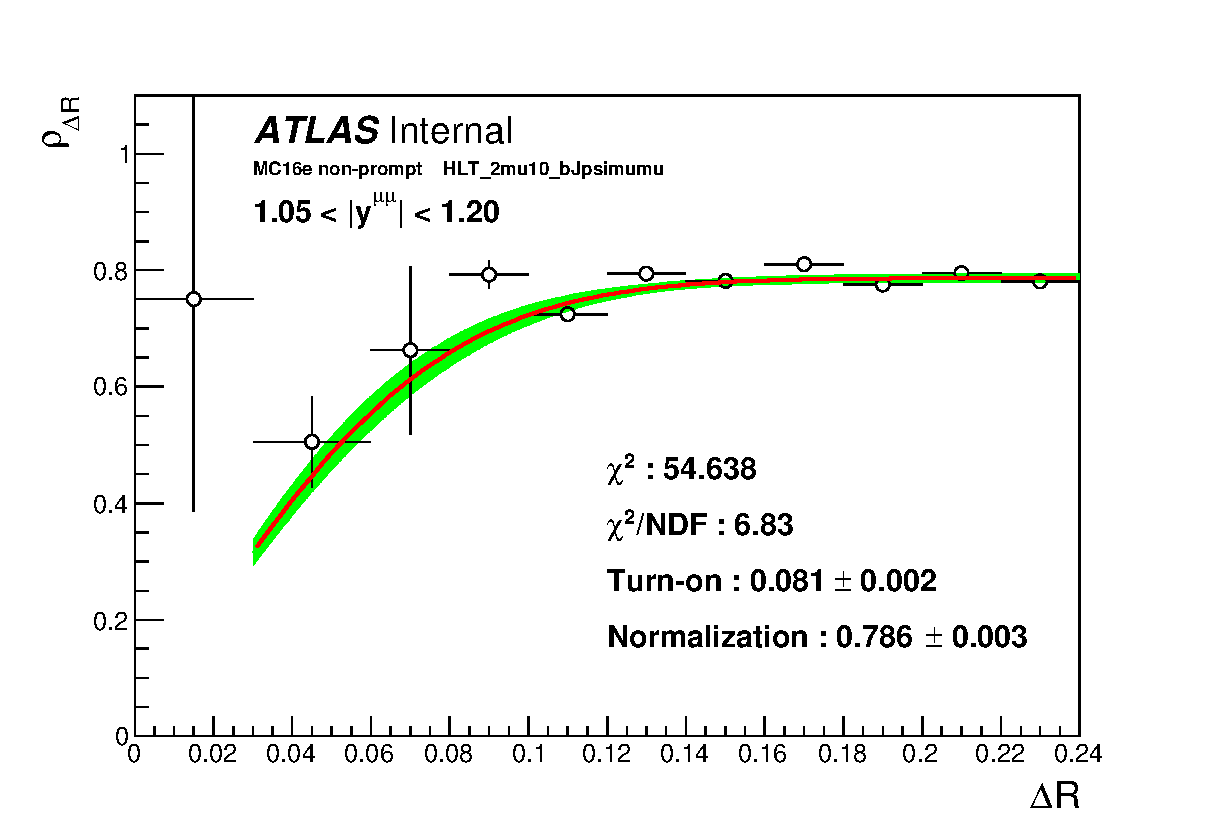
\includegraphics[width=0.33\textwidth]{htg_efficiency_Overlap_HLT_2mu10_bJpsimumu_undefined_periodMC16e} 
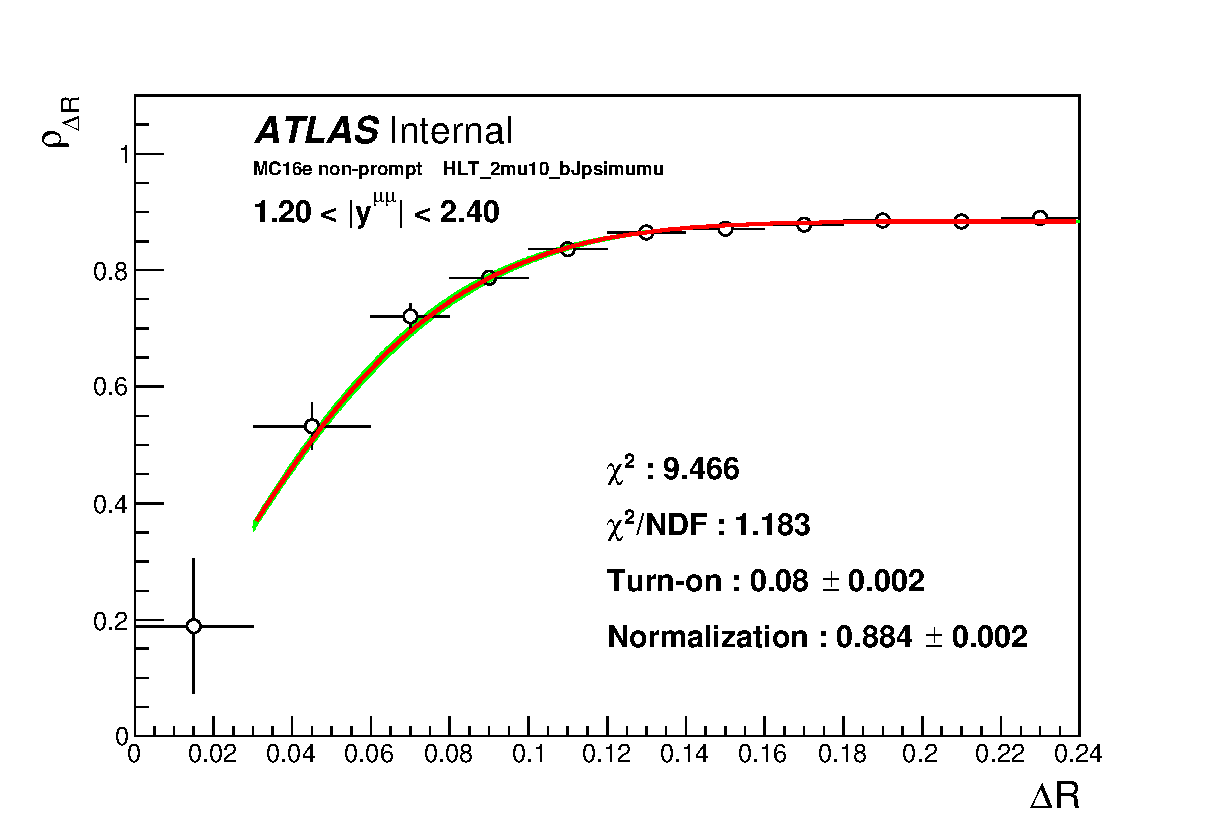
\includegraphics[width=0.33\textwidth]{htg_efficiency_Endcap_HLT_2mu10_bJpsimumu_undefined_periodMC16e} 
\caption{$\rho_{\Delta R}$ fits for \texttt{HLT\_2mu10\_bJpsimumu} in data18 (top) and MC16e (bottom)
  in the three $|y^{\mu\mu}|$ regions. The red line is the fit to the data points, and
  the green area is the uncertainty of the fit.}
\label{fig:fit_rho_dr}
\end{figure}

The true correction $c_{\Delta R}$ is extracted from the fit by removing the overall normalisation.
For $\Delta R$ smaller than the shift, $c_{\Delta R}$ is manually set to a value close to zero.
As $c_{\Delta R}$ is independent of the $p_T$ thresholds of the legs due to the additional event selection,
it is practical to extract $c_{\Delta R}$ only from \texttt{HLT\_2mu10\_bJpsimumu}
and apply it to all other di-muon triggers.
Figure~\ref{fig:c_delta_dr} shows the $c_{\Delta R}$ curves of \texttt{HLT\_2mu10\_bJpsimumu}
and \texttt{HLT\_mu11\_mu6\_bJpsimumu}. The curves of the two triggers agree very well.

\begin{figure}[h]
\center
\hspace{-0.1cm}
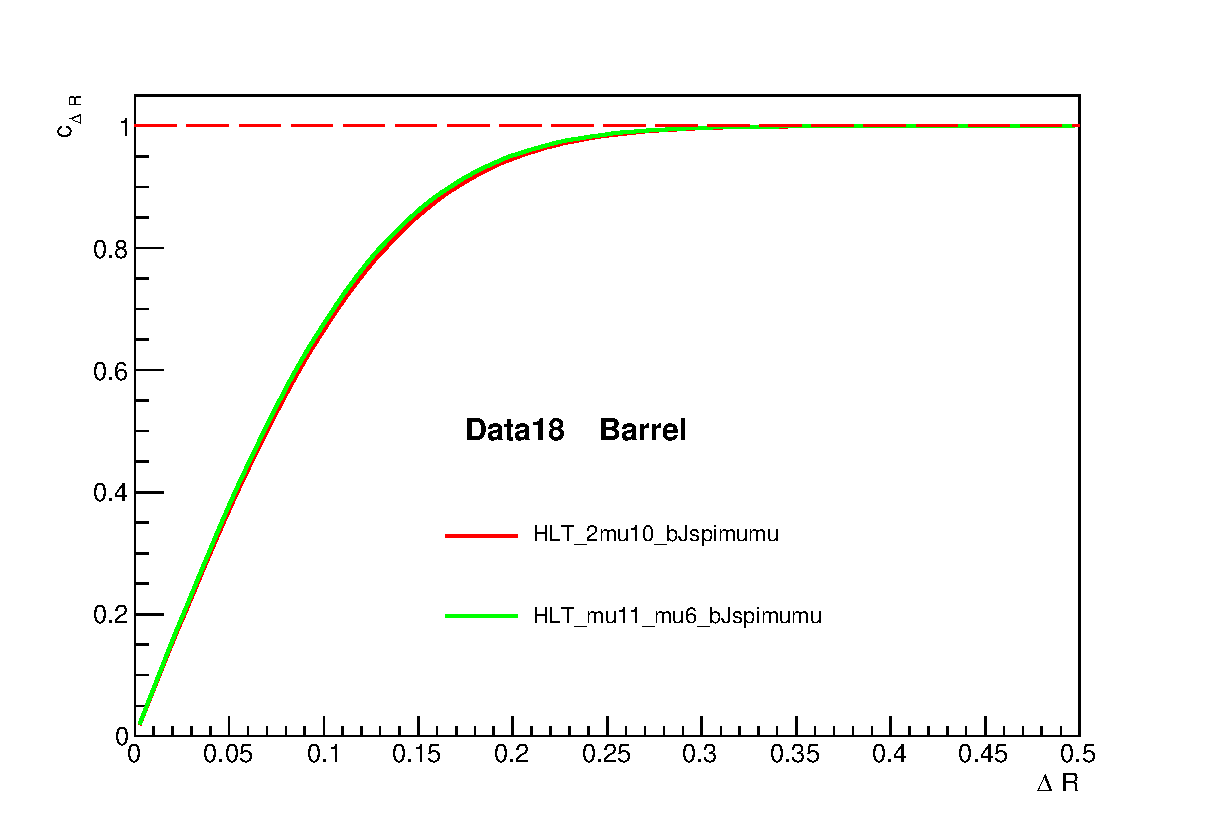
\includegraphics[width=0.33\textwidth]{c_dr_pT_thresholds_compare_Data18_Barrel.eps} 
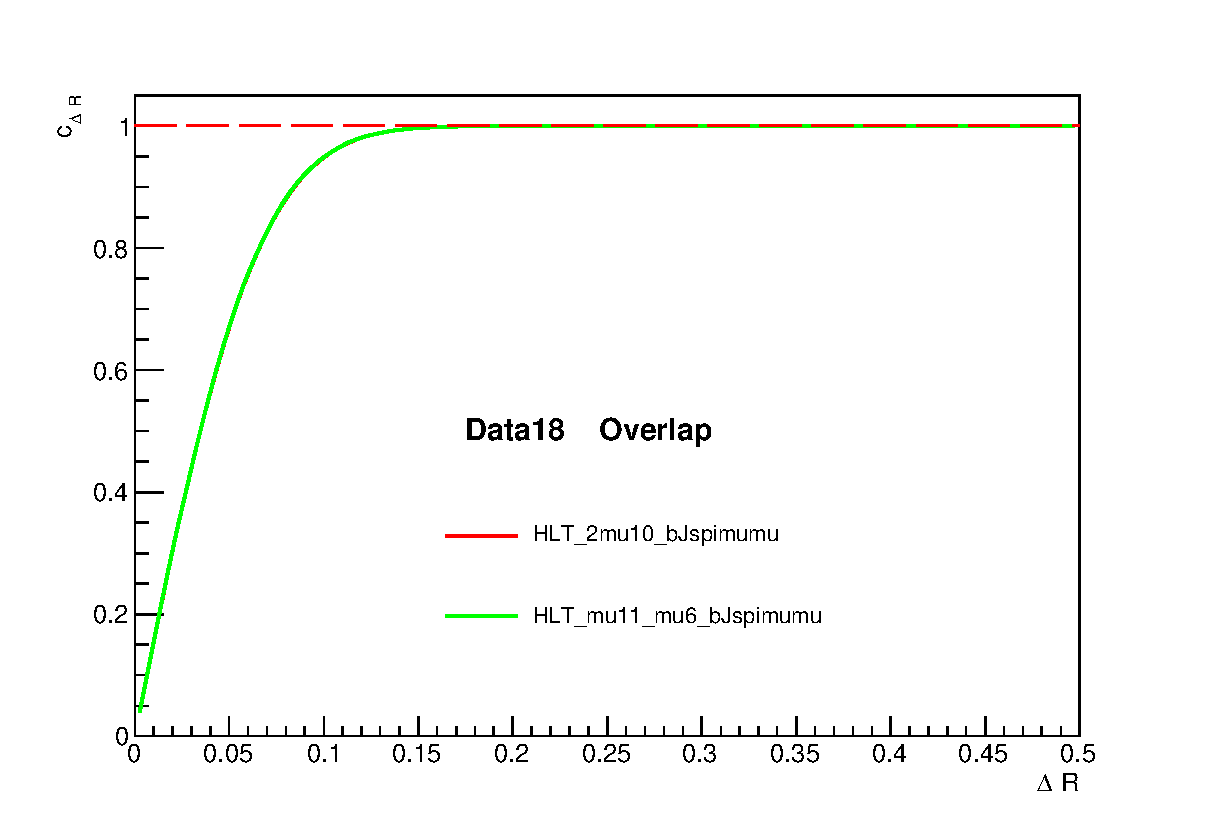
\includegraphics[width=0.33\textwidth]{c_dr_pT_thresholds_compare_Data18_Overlap.eps} 
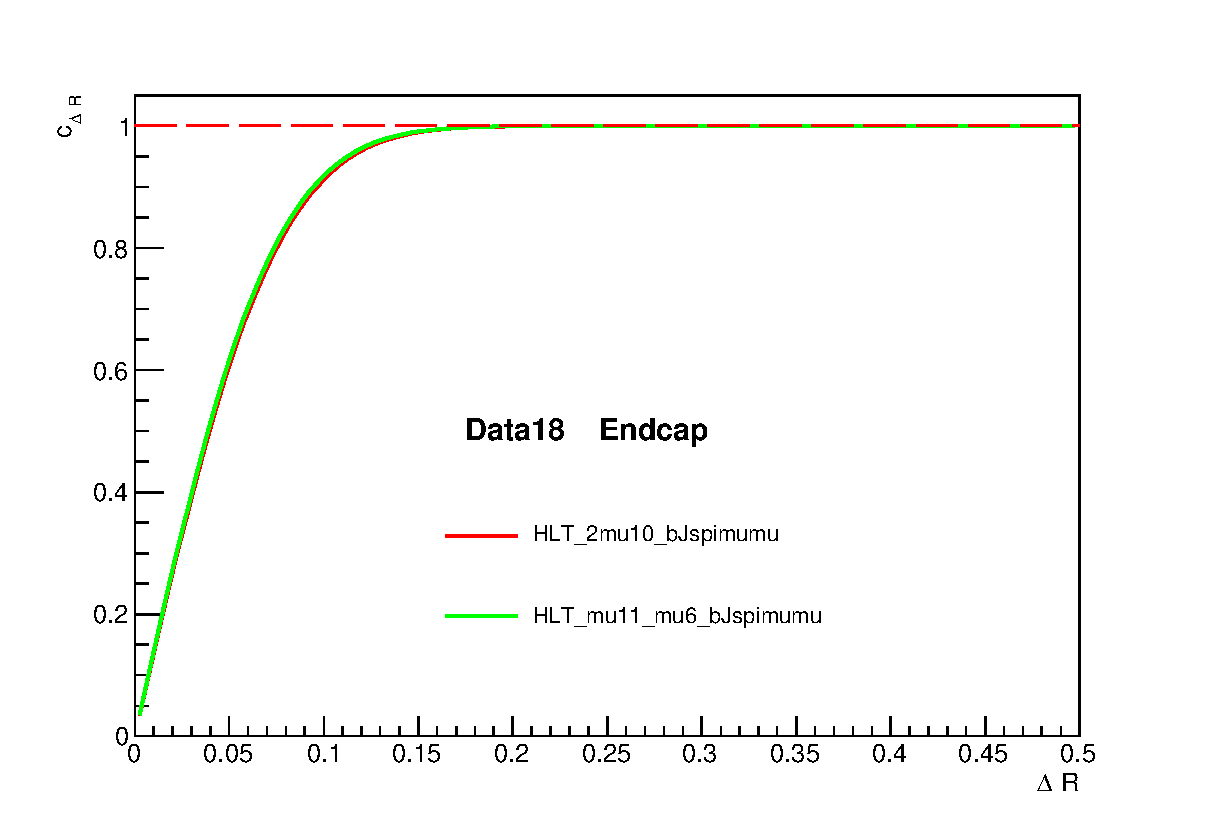
\includegraphics[width=0.33\textwidth]{c_dr_pT_thresholds_compare_Data18_Endcap.eps} \\
\hspace{-0.1cm}
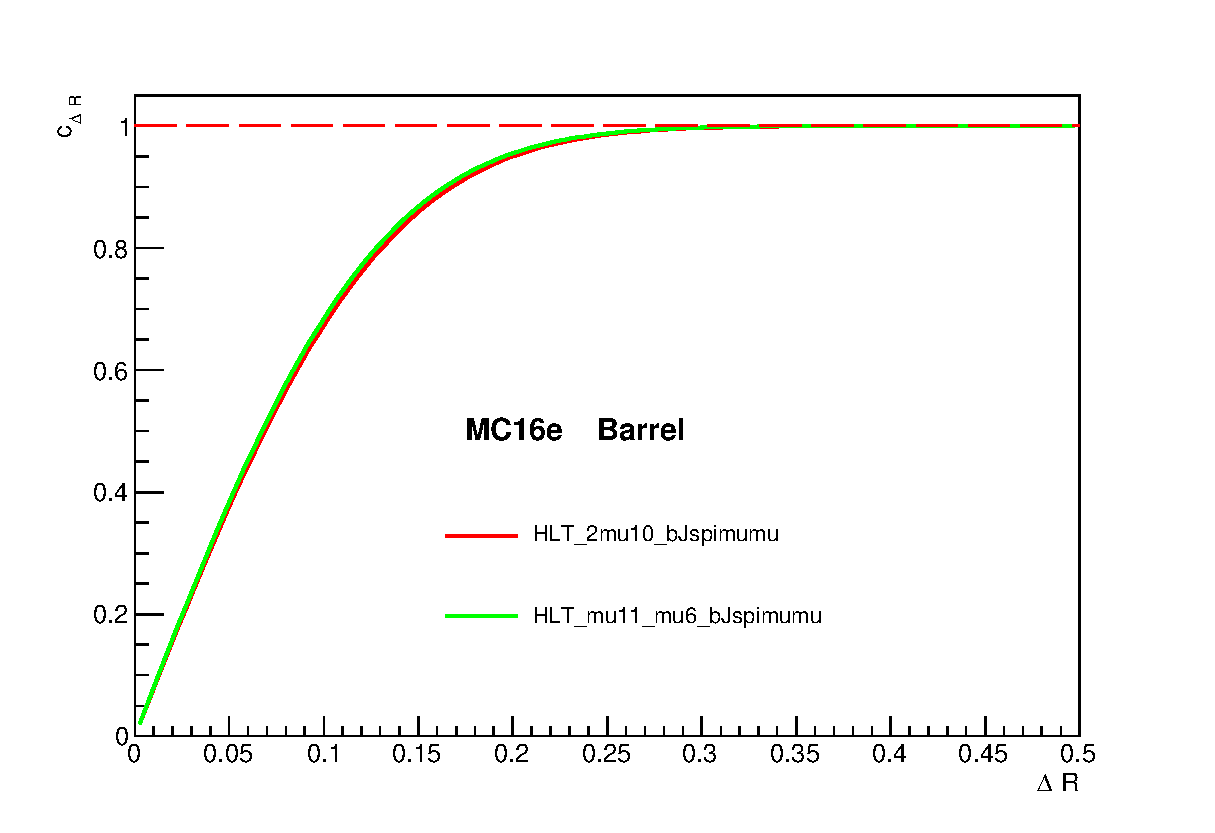
\includegraphics[width=0.33\textwidth]{c_dr_pT_thresholds_compare_MC16e_Barrel.eps} 
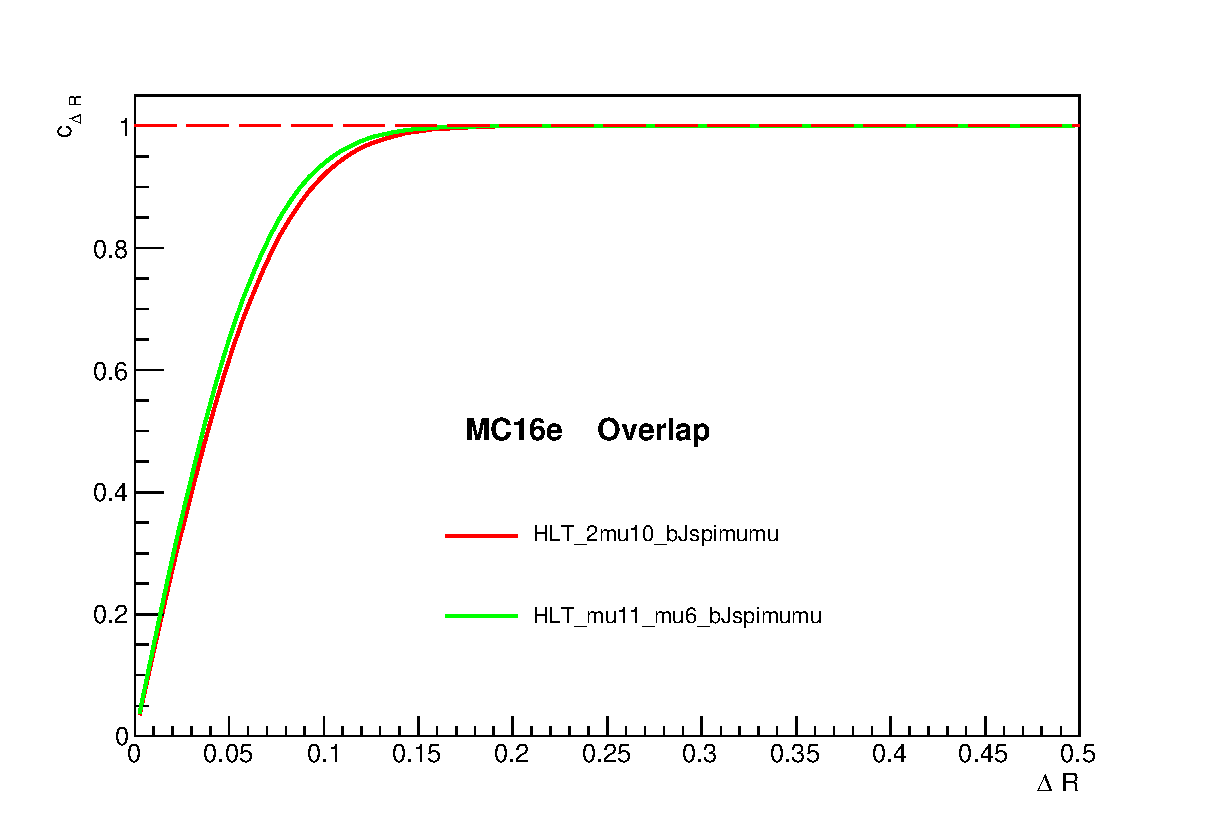
\includegraphics[width=0.33\textwidth]{c_dr_pT_thresholds_compare_MC16e_Overlap.eps} 
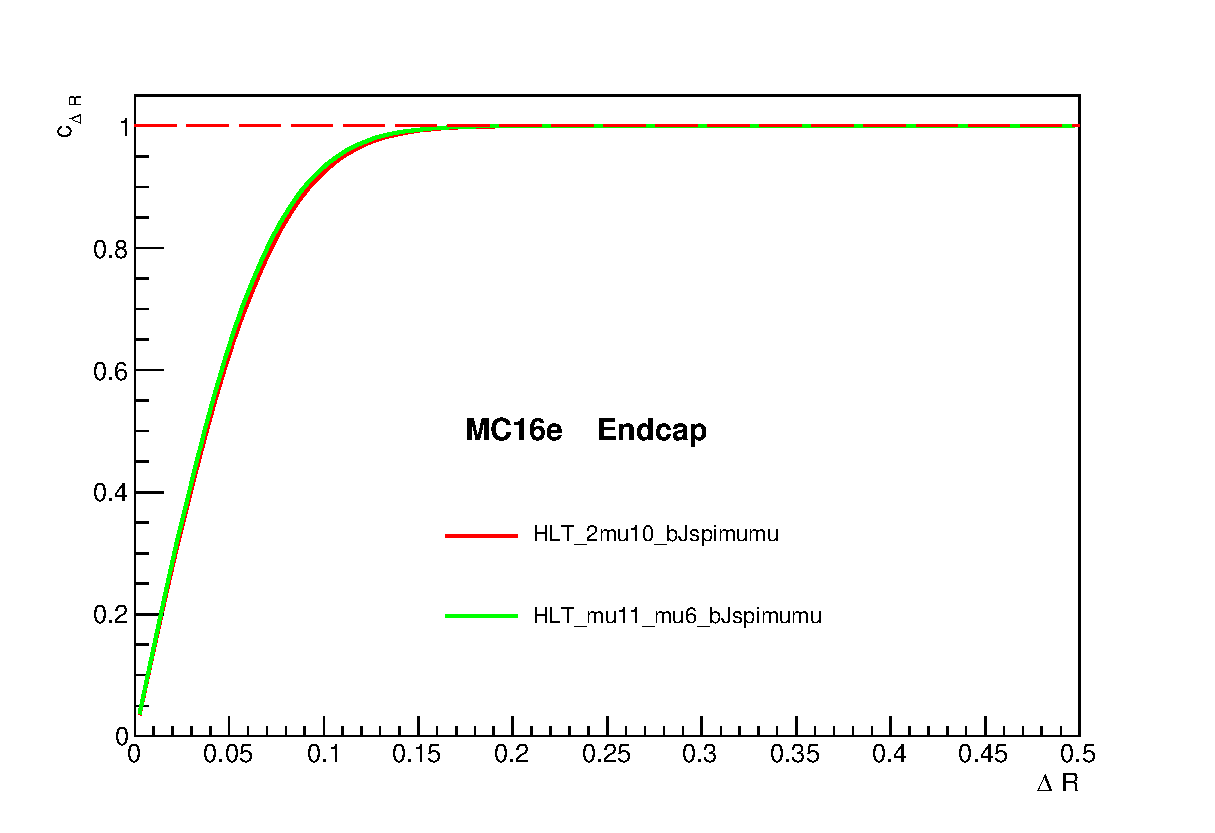
\includegraphics[width=0.33\textwidth]{c_dr_pT_thresholds_compare_MC16e_Endcap.eps} 
\caption{$c_{\Delta R}$ of \texttt{HLT\_2mu10\_bJpsimumu} and \texttt{HLT\_mu11\_mu6\_bJpsimumu} in data18 (top) and MC16e (bottom) in the three $|y^{\mu\mu}|$ regions.}
\label{fig:c_delta_dr}
\end{figure}


\subsubsection{Asymptotic correction}

The asymptotic correction $c_a$ is obtained by using an auxiliary di-muon trigger
with no vertex and opposite charge requirements, that is

\begin{equation}
c_a(|y^{\mu\mu}|) = \dfrac{N(\text{accepted by \texttt{HLT\_mu11\_mu6\_bJpsimumu}})}{N(\text{accepted by \texttt{HLT\_mu11\_mu6\_bDimu\_novtx\_noos}})}
\end{equation}

The following selections are applied:

\begin{itemize}
\item Baseline $p_T$ selection for the muons, depending on the $p_T$ thresholds of the di-muon trigger
\item Events un-prescaled with respect to the di-muon trigger
\end{itemize} 

$c_a$ saturates quickly against $\Delta R$, hence it is extracted by fitting with a constant.
In 2017-18, \texttt{HLT\_mu11\_mu6\_bDimu\_novtx\_noos} is the only available trigger
with no vertex+OS requirement. Similar to $c_{\Delta R}$, $c_a$ should not depend
on the $p_T$ thresholds of the di-muon trigger, and also $c_a$ is very close to one,
hence $c_a$ from \texttt{HLT\_mu11\_mu6\_bJpsimumu} is applied to all other triggers.
The results of the fit are shown in Figure~\ref{fig:fit_c_a}.

\begin{figure}[h]
\center
\hspace{-0.1cm}
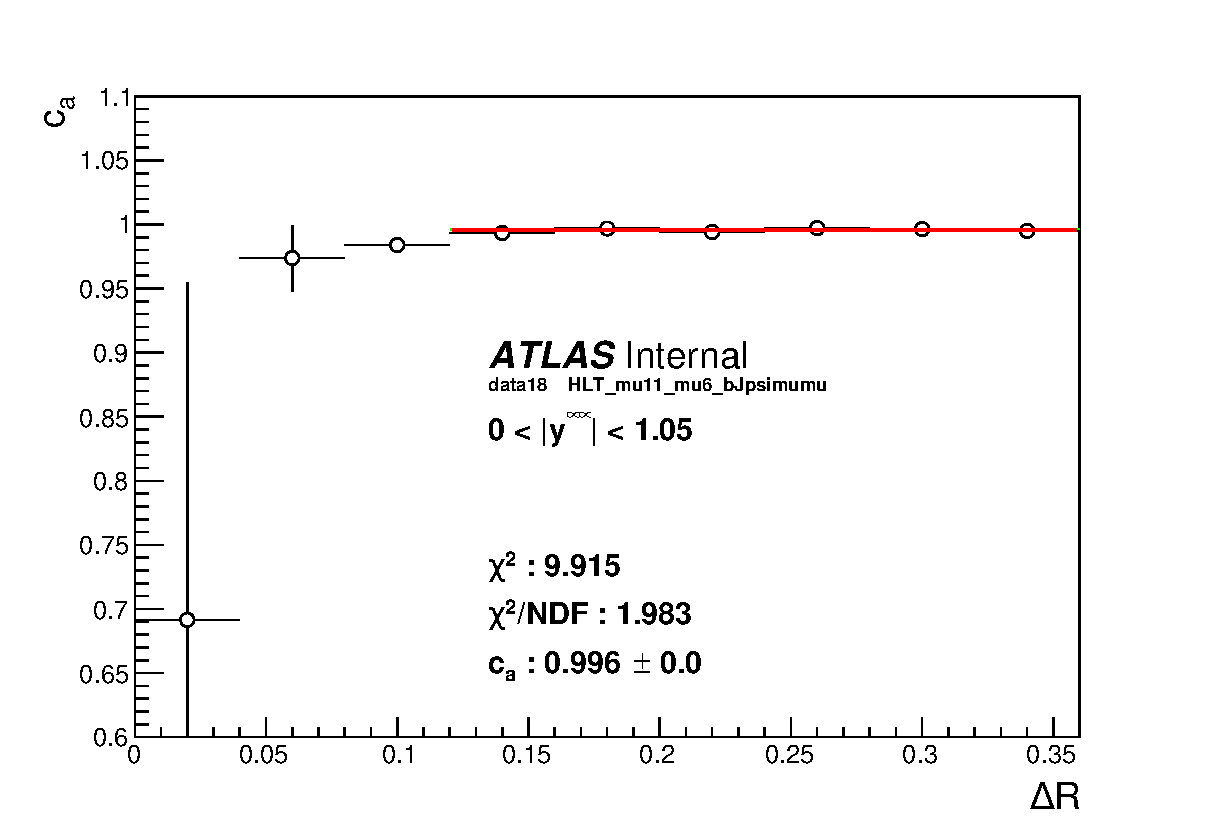
\includegraphics[width=0.33\textwidth]{plots_fit_c_a_data18_Barrel.eps} 
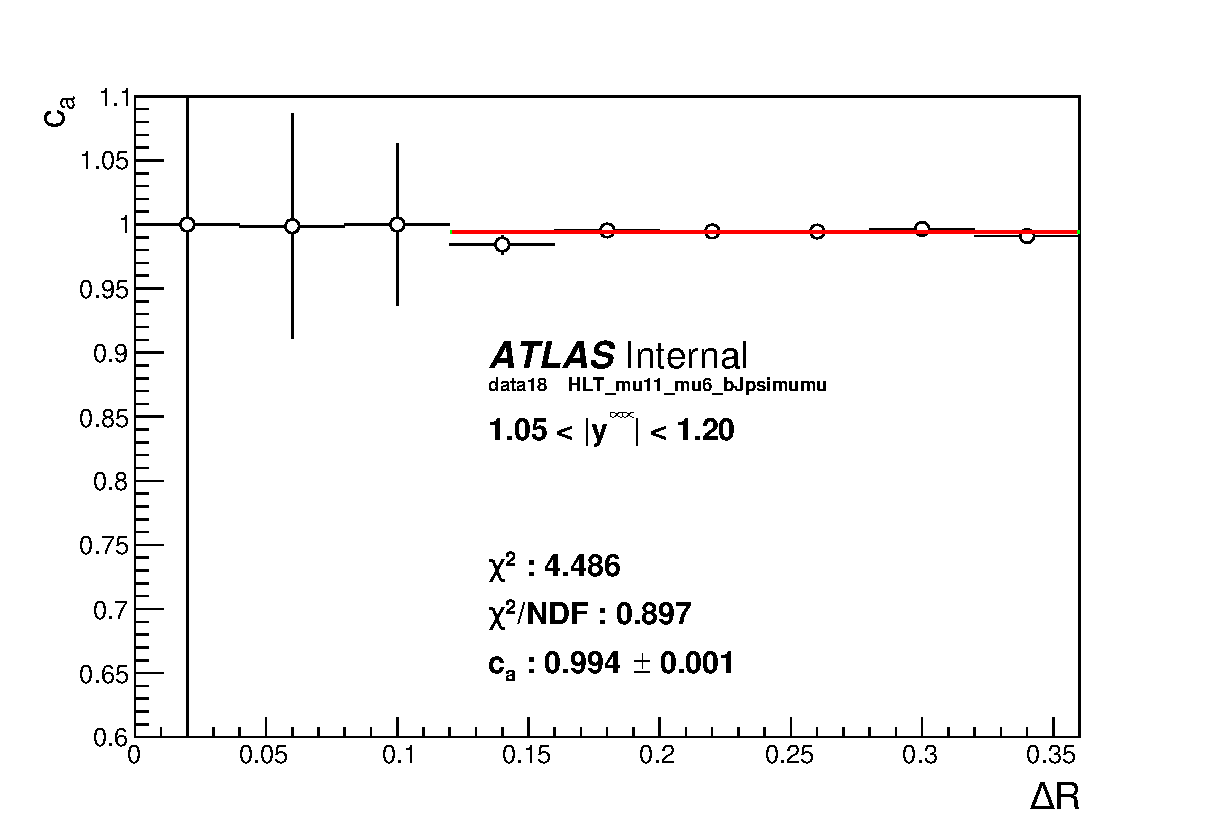
\includegraphics[width=0.33\textwidth]{plots_fit_c_a_data18_Overlap.eps} 
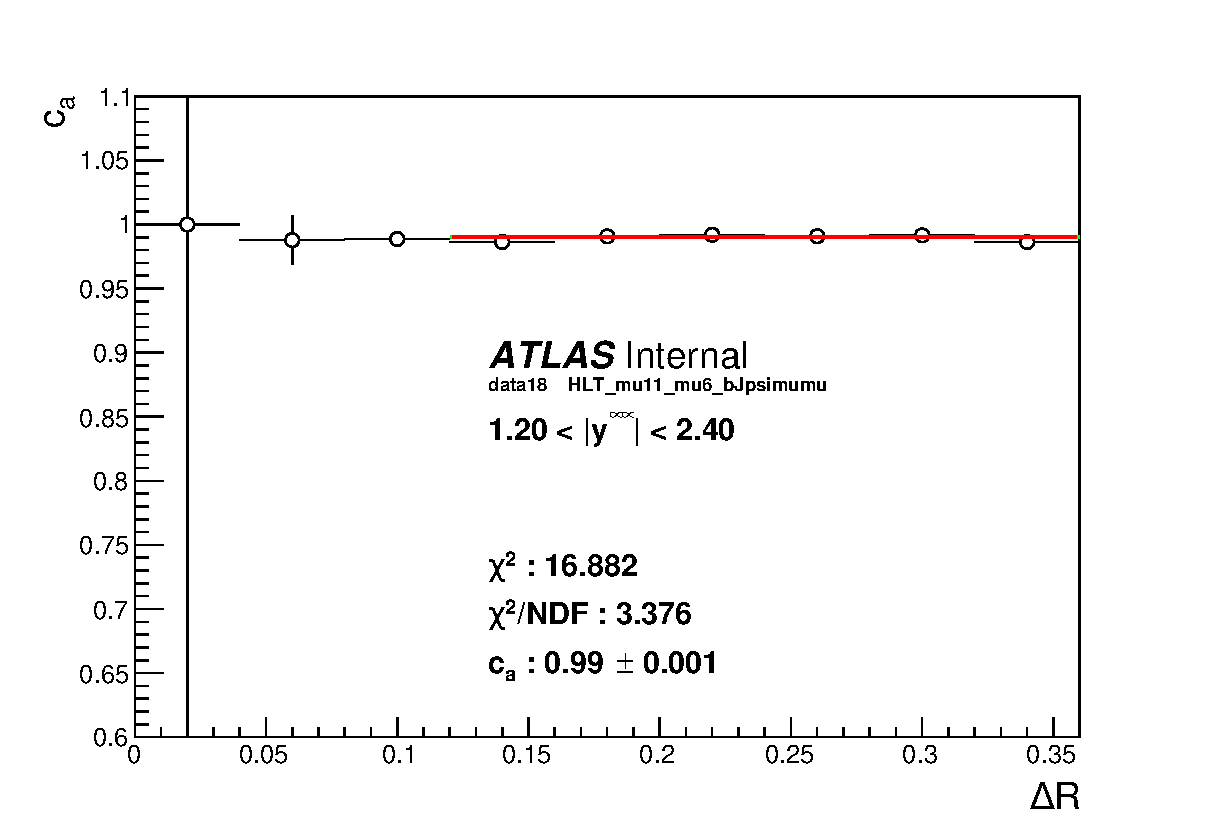
\includegraphics[width=0.33\textwidth]{plots_fit_c_a_data18_Endcap.eps} \\
\hspace{-0.1cm}
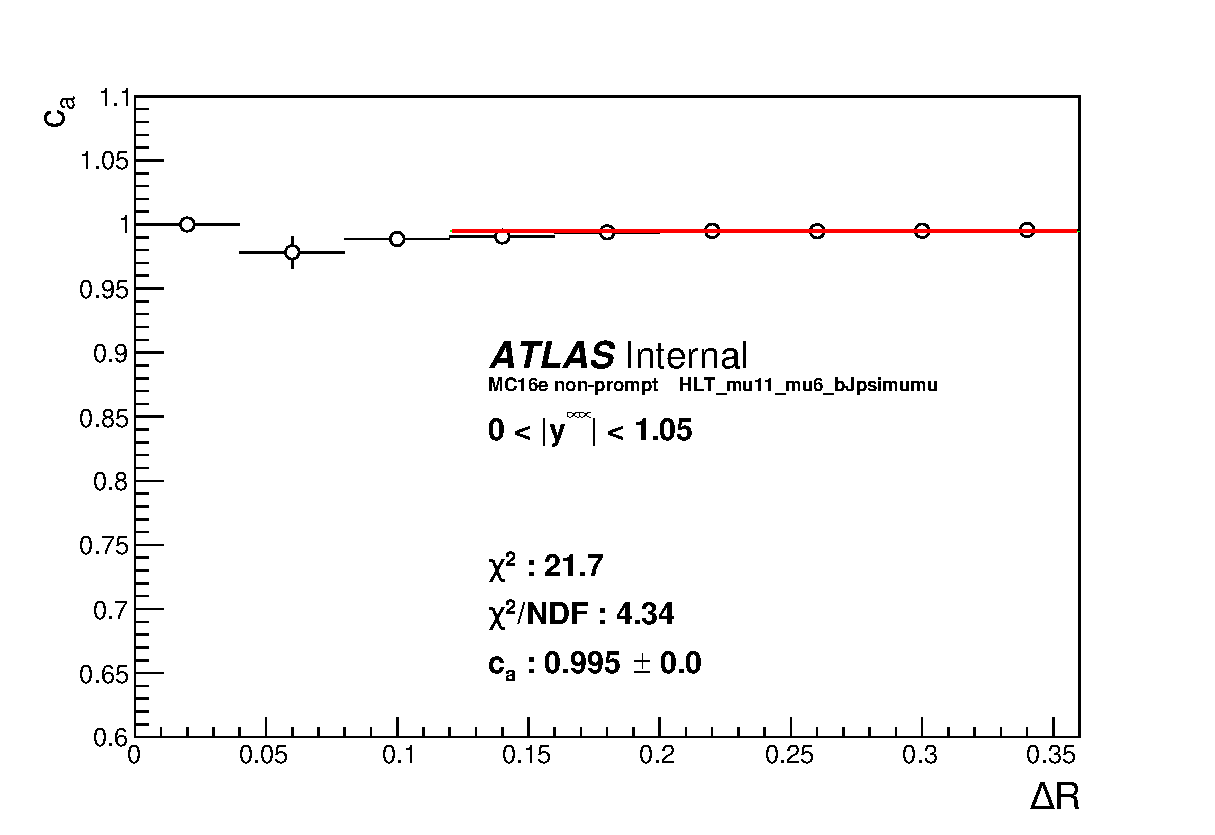
\includegraphics[width=0.33\textwidth]{plots_fit_c_a_mc16e_Barrel.eps} 
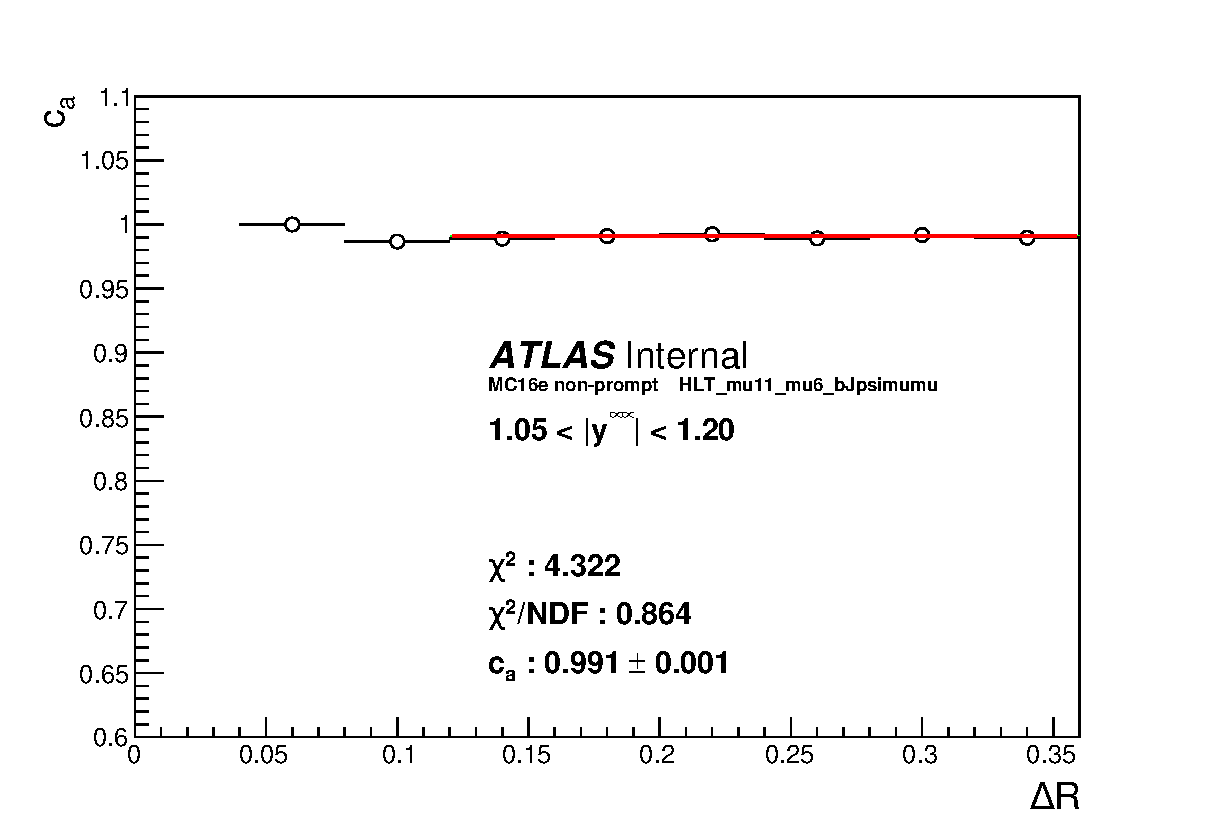
\includegraphics[width=0.33\textwidth]{plots_fit_c_a_mc16e_Overlap.eps} 
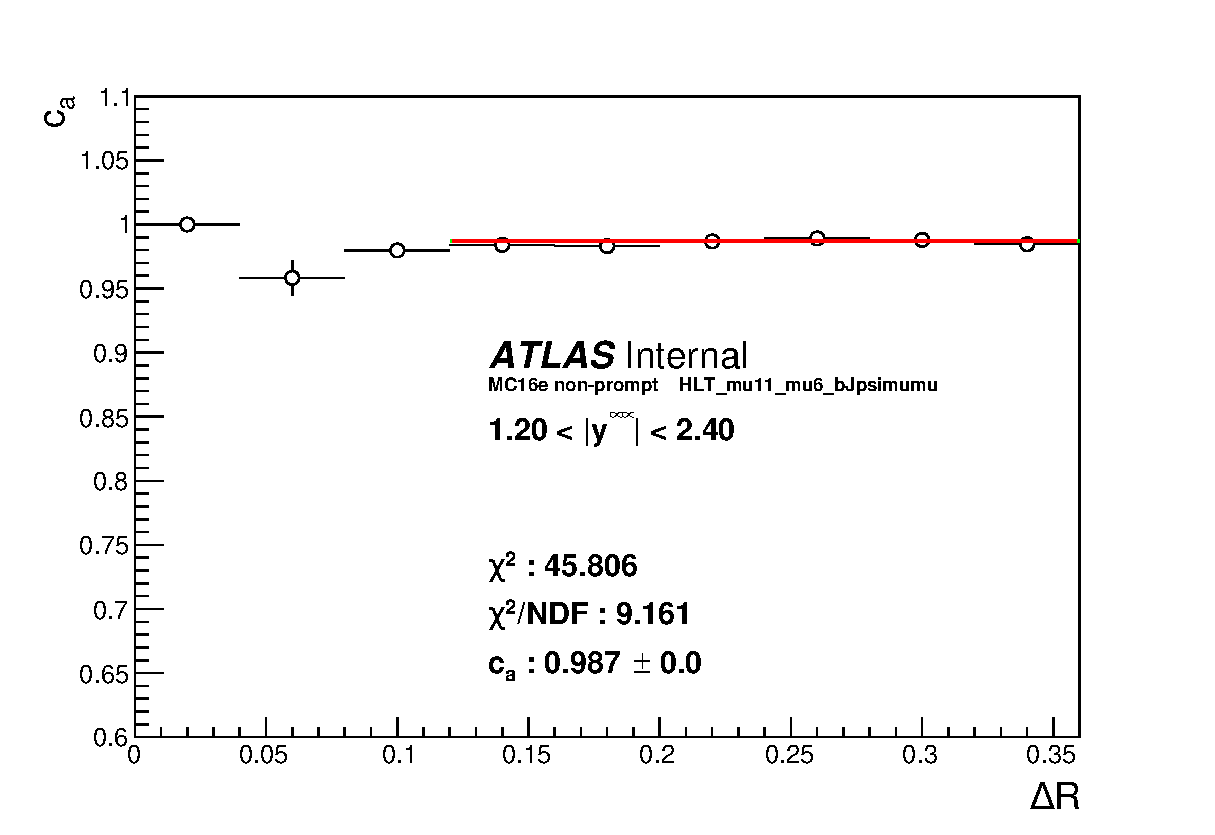
\includegraphics[width=0.33\textwidth]{plots_fit_c_a_mc16e_Endcap.eps} 
\caption{$\rho_{\Delta R}$ fits for \texttt{HLT\_2mu10\_bJpsimumu} in data18 (top)
  and MC16e (bottom) in the three $|y^{\mu\mu}|$ regions. The red line is the fit
  to the data points, and the green area is the uncertainty of the fit.}
\label{fig:fit_c_a}
\end{figure}


\subsubsection{Single muon efficiency}

The single muon efficiency is obtained using the same method as Run 1.
To extract, for example, the single muon efficiency of \texttt{HLT\_mu10\_nomucomb}, we first obtain the ratio:

\begin{equation}
  \rho_{J/ \psi}(p^{\text{probe}}_T, q\eta^{\text{probe}}, \Delta R, |y^{\mu\mu}|)
  = \dfrac{N(\text{tagged + accepted by \texttt{HLT\_2mu10\_bJpsimumu}})}{N(\text{tagged by \texttt{HLT\_mu10\_bJpsi\_TrkPEB}})}
\end{equation}

The single muon efficiency can then be extracted by weighting $\rho_{J/ \psi}$
by the reciprocal of the di-muon correction $c_{\mu\mu}$:

\begin{equation}
\varepsilon_{\text{mu10}}(p_T, q\eta) = \dfrac{\rho_{J/ \psi}(p_T, q\eta, \Delta R, |y^{\mu\mu}|)}{c_{\mu\mu}(\Delta R, |y^{\mu\mu}|)}
\end{equation}

In 2018, un-prescaled, non-L1topo and symmetric \texttt{2mu6} triggers are not available.
Hence, $\varepsilon_{\text{mu6}}$ can only be obtained from asymmetric
\texttt{HLT\_mu11\_mu6\_bJpsimumu} trigger. However, it is difficult to determine whether
the probe muon matches to the mu11 leg or the mu6 leg.
To increase the chance that the tag muon is accepted by the mu11 leg and the probe muon
is matched to the mu6 leg, the following selections are added:

\begin{itemize}
\item Tag muon matched to \texttt{HLT\_mu10\_bJpsi\_TrkPEB} and tag $p_T > 11 \text{ GeV}$
\item For probe $p_T < 11 \text{ GeV}$, the probe muon should be simultaneously accepted
  or rejected by both \texttt{HLT\_mu6\_nomucomb} and \texttt{HLT\_mu11\_mu6\_bJpsimumu}
\end{itemize} 

Figure~\ref{fig:Run1_singlemueffmap} shows the 2D maps of efficiency in terms of $p_T$ and $q\eta$. 


\begin{figure}[h]
\center
\hspace{-0.5cm}
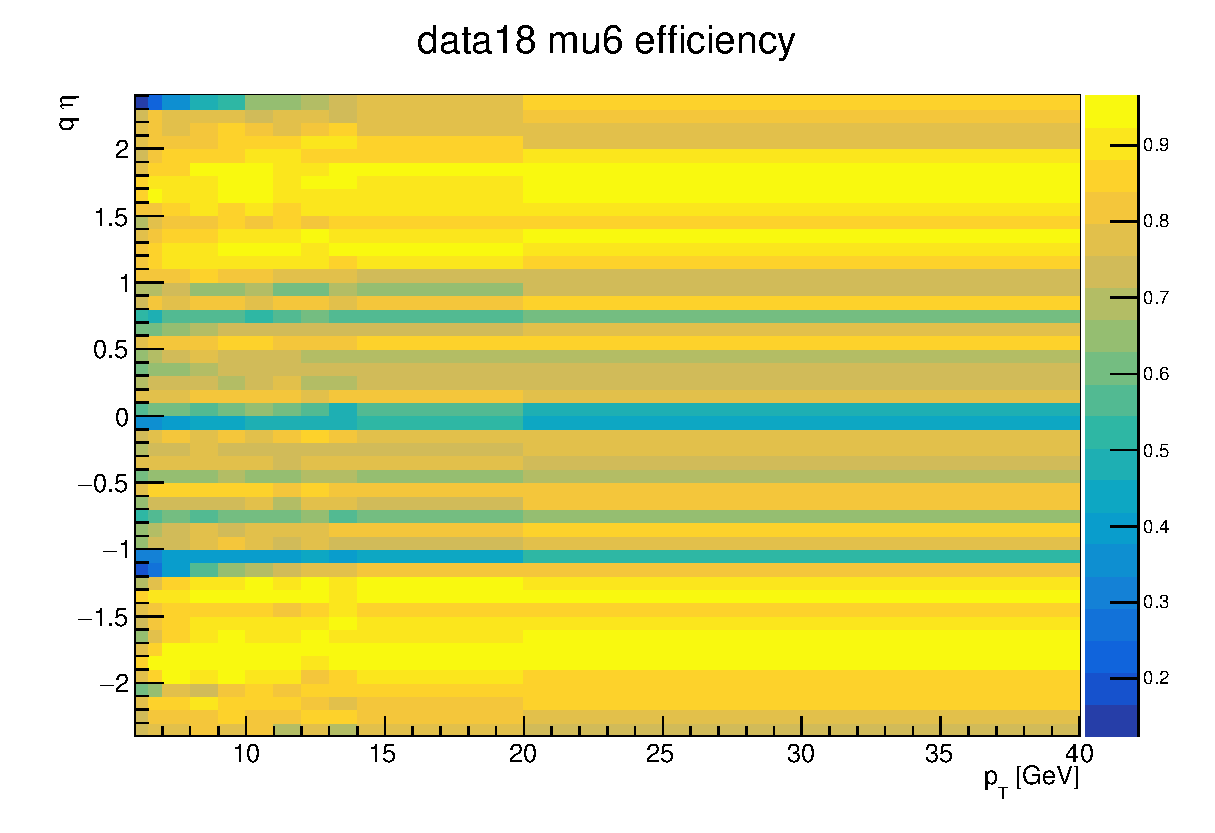
\includegraphics[width=0.5\textwidth]{Run1_data18_mu6.eps} 
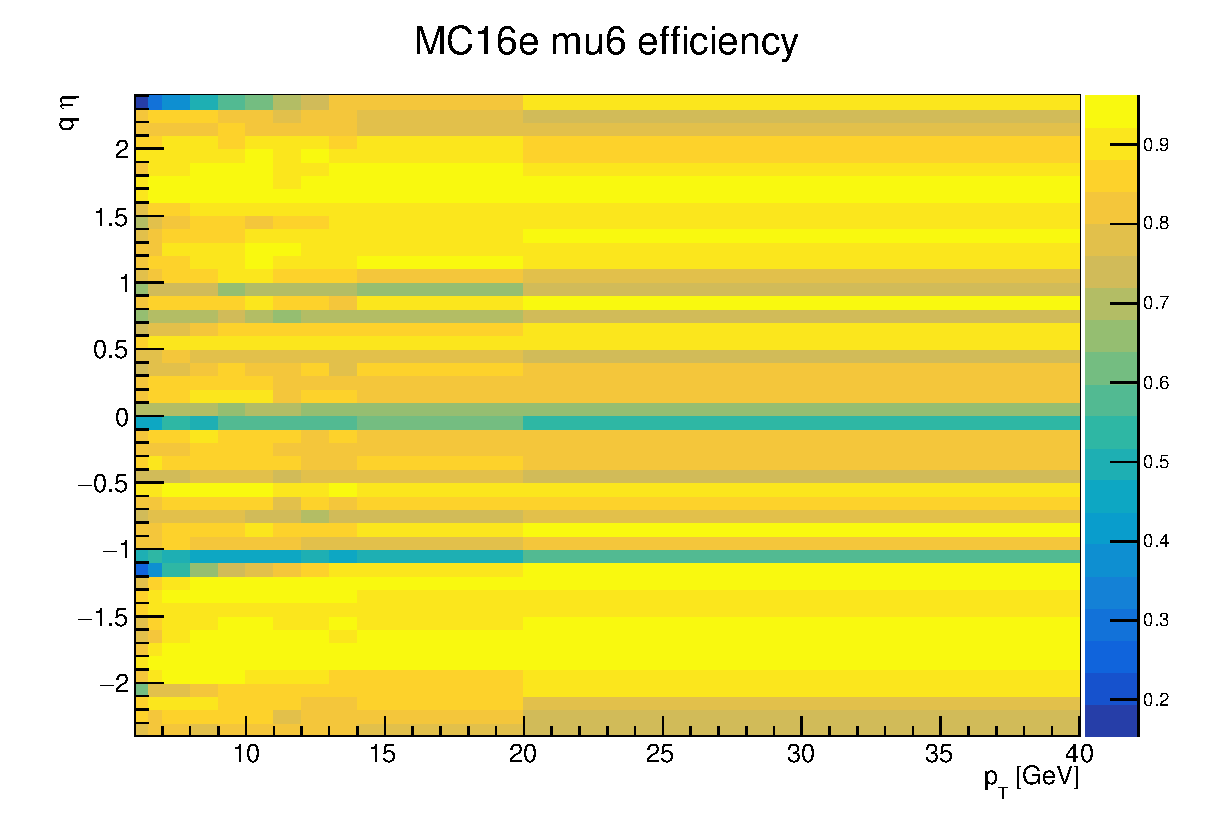
\includegraphics[width=0.5\textwidth]{Run1_MC16e_mu6.eps} 
\caption{The maps of single muon efficiency of \texttt{HLT\_mu6\_nomucomb} extracted by
  the Run-1 method using \texttt{HLT\_mu11\_mu6\_bJpsimumu} as the di-muon trigger.}
\label{fig:Run1_singlemueffmap}
\end{figure}

%-------------------------------------------------------------------------------
\section{Event Selection}
\label{sec:selection}
%-------------------------------------------------------------------------------

\subsection{Event Preselection}
\label{sec:preselection}
The work flow for event selection is as follows.
Firstly the data (or Monte Carlo) collections are run over using an Athena job on the Grid.
This performs basic event reconstruction and is followed by the preselection stage.
We use release XX.XX to process the data.
The preselection software can be found in the package XX.
%The post-Athena processing code can be found in the ntuple subdirectory of the package.

In the Athena reconstruction, as a first step a JpsiFinder tool is run on muon or electron
containers, searching for di-lepton candidates with opposite sign and invariant mass
in the range [0, 6000] \mev. The \pt of the Leptons is required to be $> 2$ \gev.
%Di-lepton candidates are considered if the vertex $\chisqr$ per degree of freedom is
%$\chisqr < 30$.

\Bd candidates are then formed by BCompositeParticleBuilder [??] tool from two tracks associated
with leptons with $\pt > 500$ [??] \mev and two other opposite-signed tracks not identified as muons
or electrons (i.e. hadrons from $K^*$ candidates). These four tracks are fitted into \Bd vertex
with track mass hypotheses set for \Bd and \Bdb (kaon mass assigned to positive or negative track).
Secondary \Bd and \kstar vertices are re-fitted using TrkVKalVrtFitter [???], primary vertices
are refitted without the four candidate tracks and additional cuts are applied: 
%{\red Q) What type of fit is performed and are there any constraints used in the fit?}
\begin{itemize}
\setlength{\itemsep}{0pt}%
\setlength{\parskip}{0pt}%
 \item \Bd or \Bdb vertex $\chisqr < 205$, [??]
 \item \Bd or \Bdb mass in the range [3000, 6000] \mev, [??]
 \item \kstar or \akstar mass in the range [600, 1050] \mev. [??]
\end{itemize}

Events are saved in a linked per-event tree with one \kstar/\akstar\ candidate for each \Bd candidate:
both possible $K^\pm\pi^\pm$ assignments are considered when dealing with combinatorics and
this results in multiple candidates per event.

For the reconstruction of primary vertex (PV), the PV of the \Bd candidate is chosen to be
the one closest to the reconstructed decay vertex of the \Bd or \Bdb candidate using the three-dimensional
distance.

After the Athena reconstruction described above, a preselection is applied:
\begin{itemize}
\setlength{\itemsep}{0pt}%
\setlength{\parskip}{0pt}%
 \item opposite charged lepton pairs and hadron pairs
 \item $\Delta R_{ee} \geq 0.1$
 \item \pt(leptons)$\geq 5$~\gev
 \item $|\eta|$(leptons)$\leq 2.5$
 \item \pt(hadrons)$\geq 0.5$~\gev
 \item $|\eta|$(hadrons)$\leq 2.5$
 \item $m(ee)\leq 7$~\gev
 \item $m(K\pi ee) \in [3000,6500]$~\mev
 \item $m(K\pi) \in [690, 1110]$~\mev
 \item Track Quality requirements on all four tracks and ID requirements on electrons
% \item $|m(K\pi)-m(K^{0*})|\leq 50$~\mev
%\item \Bd$(\chisqr) \leq 2$
%\item $\tau$(\Bd)$\geq 0.2$~ps
\end{itemize}

The cut flow from this preselection for signal events ($\Bd \to \kstar ee$) and resonance events
($\Bd \to J/\psi(ee)\kstar$) are shown in Tables~\ref{tab:presel:sigele} and~\ref{tab:presel:resele}
for the electron final state.

\begin{table}[!ht] 
\caption{Number of events surviving the pre-selection for the signal non-resonant sample for the electron final state.} 
\centering 
\hspace*{-1.cm}
{\small
\begin{tabular}{l | l l l l l l l l l } 
\hline\hline
Selection &             &        & Truth- & Truth- & Relative & Relative &  &  Ratio of\\
criterion & Candidates  & Events & matched & matched & efficiency & efficiency & Purity & relative \\
          &             &        & candidates & events &          & (truth- & & efficiencies\\
          &             &        &   &   &          & matched) & & \\        
\hline
   to     &    be       &  filled      &   &   &          & & & \\        
\hline\hline
\end{tabular} 
}
\label{tab:presel:sigele}
\end{table}


\begin{table}[!ht] 
\caption{Number of events surviving the pre-selection for the reference resonant sample for the electron final state.} 
\centering 
\hspace*{-1.cm}
{\small
\begin{tabular}{l | l l l l l l l l l } 
\hline\hline
Selection &             &        & Truth- & Truth- & Relative & Relative &  &  Ratio of\\
criterion & Candidates  & Events & matched & matched & efficiency & efficiency & Purity & relative \\
          &             &        & candidates & events &          & (truth- & & efficiencies\\
          &             &        &   &   &          & matched) & & \\        
\hline
baseline & 2515085 & 217958 & 156485 & 154886 &  &  &   0.711 &  \\
$\pT(\ell_1)>5$~GeV & 2515085 & 217958 & 156485 & 154886 &  1.000 &  1.000 &  0.711 &  1.000 \\
$\pT(\ell_2)>5$~GeV & 2515085 & 217958 & 156485 & 154886 &  1.000 &  1.000 &  0.711 &  1.000 \\
$\eta(\ell_1)<2.5$ & 2515085 & 217958 & 156485 & 154886 &  1.000 &  1.000 &  0.711 &  1.000 \\
$\eta(\ell_2)<2.5$ & 2515085 & 217958 & 156485 & 154886 &  1.000 &  1.000 &  0.711 &  1.000 \\
$\pT(h_1)>1$~GeV & 913674 & 195110 & 121550 & 120286 &  0.895 &  0.777 &  0.617 &  0.868 \\
$\pT(h_2)>1$~GeV & 417361 & 153585 & 99455 & 98392 &  0.787 &  0.818 &  0.641 &  1.039 \\
$\eta(h_1)<2.5$ & 416603 & 153460 & 99312 & 98252 &  0.999 &  0.999 &  0.640 &  0.999 \\
$\eta(h_2)<2.5$ & 415912 & 153329 & 99192 & 98134 &  0.999 &  0.999 &  0.640 &  1.000 \\
$\chi^2(B)/$NDoF$<2$ & 286407 & 131015 & 88514 & 87592 &  0.854 &  0.893 &  0.669 &  1.045 \\
$\tau(B)>0.2$ & 207721 & 109944 & 77542 & 76747 &  0.839 &  0.876 &  0.698 &  1.044 \\
\hline
$|\Delta m(K\pi)_\mathrm{PDG}| < 50$~MeV & 59235 & 49955 & 29008 & 28765 &  0.454 &  0.375 &  0.576 &  0.825 \\
$m(B)\in [4.7,5.7]$~GeV & 43969 & 40179 & 26654 & 26447 &  0.804 &  0.919 &  0.658 &  1.143 \\
\hline
$|\Delta m(\pi K)_\mathrm{PDG}| < 50$~MeV & 59689 & 50276 & 29148 & 28868 &  0.457 &  0.376 &  0.574 &  0.823 \\
$m(\overline{B})\in [4.7,5.7]$~GeV & 44390 & 40545 & 26724 & 26473 &  0.806 &  0.917 &  0.653 &  1.137 \\
\hline
best $\chi^2(B)$ & 64742 & 64742 & 51785 & 51785 &  1.597 &  1.956 &  0.800 &  1.225 \\
\hline\hline
\end{tabular} 
}
\label{tab:presel:resele}
\end{table}


The cut flow from this preselection for signal events ($\Bd \to \kstar \mu\mu$) and resonance events
($\Bd \to J/\psi(\mu\mu)\kstar$) are shown in Tables~\ref{tab:presel:sigmu} and~\ref{tab:presel:resmu}
for the muon final states.

\begin{table}[!ht] 
\caption{Number of events surviving the pre-selection for the signal non-resonant sample for the muon final state.} 
\centering 
\hspace*{-1.cm}
{\small
\begin{tabular}{l | l l l l l l l l l } 
\hline\hline
Selection &             &        & Truth- & Truth- & Relative & Relative &  &  Ratio of\\
criterion & Candidates  & Events & matched & matched & efficiency & efficiency & Purity & relative \\
          &             &        & candidates & events &          & (truth- & & efficiencies\\
          &             &        &   &   &          & matched) & & \\        
\hline
   to     &    be       &  filled      &   &   &          & & & \\        
\hline\hline
\end{tabular} 
}
\label{tab:presel:sigmu}
\end{table}


\begin{table}[!ht] 
\caption{Number of events surviving the pre-selection for the reference resonant sample for the muon final state.} 
\centering 
\hspace*{-1.cm}
{\small
\begin{tabular}{l | l l l l l l l l l } 
\hline\hline
Selection &             &        & Truth- & Truth- & Relative & Relative &  &  Ratio of\\
criterion & Candidates  & Events & matched & matched & efficiency & efficiency & Purity & relative \\
          &             &        & candidates & events &          & (truth- & & efficiencies\\
          &             &        &   &   &          & matched) & & \\        
\hline
   to     &    be       &  filled      &   &   &          & & & \\        
\hline\hline
\end{tabular} 
}
\label{tab:presel:resmu}
\end{table}


The percentage of multiple candidates after the preselection is about XX\% (XX\%)
for signal (resonance) simulated events.








\subsection{Multiple Candidates}
Due to the four-particle final states and the unavailability of $K/\pi$ separation,
there is a significant number of events with multiple candidates.

Hence we can include two further stages of selection in order to
obtain a single candidate per event, which can be useful for various tests.
As mentioned above, each event consists of multiple \Bd~candidates, and each candidate has
two possible mass hypotheses, i.e., whether an individual candidate corresponds to a \Bd or \Bdb.
To select amongst different four-particle sets, the single best four-particle set per event is
chosen based on the best $\chi^2$/Nd.o.f., referred to as the best-$\chi^2$ selection.

After the best-$\chi^2$ selection, we can still have two candidates corresponding to the two
hadron assigments ($K\pi$ and $\pi K$), Hence we can assign a single reconstructed mass to
the selected four-track set choosing between the two mass hypotheses (as the switching of
the $K$ and $\pi$ tracks lead to a change in the reconstructed $B$ mass).
The assignment of the $B$ mass is done in two ways: a comparison to the $K^*$ mass PDG value
is done and the closer of the two hypotheses is chosen, or in the gNN architecture,
a multi-class gNN produces a classification score for each candidate as \Bd, \Bdb, and background
and the highest of these is chosen.
The former of these is referred to as the best-$K^*$ mass selection.

The two additional selections above (the best-$\chi^2$ and the best-$K^*$ mass) are labelled
the best-candidate selection in the following and in the cutflow
tables~\ref{tab:presel:sigele},~\ref{tab:presel:resele},~\ref{tab:presel:sigmu} and~\ref{tab:presel:resmu}.


The percentage of events with more than one four-particle sets before the preselection is about $84.2\%$ ($82.1\%$)
for the non-resonant (resonant) sample for the electron final state,
while the same percentage after the preselection is down to about $18.7\%$ ($23.3\%$)
for the non-resonant (resonant) sample for the electron final state.

The percentage of events with more than one candidate before the preselection is about $73.2\%$ ($71.8\%$)
for the non-resonant (resonant) sample for the muon final state,
while the same percentage after the preselection is down to about $46.5\%$ ($42.1\%$)
for the non-resonant (resonant) sample for the muon final state.

\begin{table}[h]
\begin{center}
\begin{tabular}{cccccc}
\hline
            &  \% of events with           &  \% of events with  \\
            &  $\geq 1$ four-particle sets &  $\geq 1$ candidate \\
\hline\hline
electron final states   & & \\
\hline
~~~~non-resonant signal & $18.7\%$  & \\
~~~~resonant $J/\psi K^*$ & $23.3\%$ & \\
\hline\hline
muon final states       & & \\
\hline
~~~~non-resonant signal & & $46.5\%$ \\
~~~~resonant $J/\psi K^*$ &  & $42.1\%$ \\
\hline\hline
\end{tabular}
\end{center}
\caption{Percentages of multiple candidates after pre-selection in both the non-resonant and
resonant MC samples.}
\label{tab:multiplecandidates}
\end{table}











\subsection{Continuum Reduction Selection}
While the main strategy for signal extraction uses Multivariate algorithms, but
we have optimised a basic selection using standard discriminating variables
that can be used for increasing the signal-over-background ratio for various studies.

% - Description of the background
The background is made up of two distinctly behaving components: combinatorial background
and \lq B-like\rq\, background. The combinatorial background arises from the random
combination of unrelated tracks in the detector. The \lq B-like\rq\, decays arise from
similar decays involving B mesons, in which one or more of the final state particles
are misidentified and so lead to the event being reconstructed as a $B_{d}^{0} \xrightarrow{} K^{*}e^{+}e^{-}$ event.
One problem, however, is that the background events consist of an overwhelming combinatorial component,
this component of the background is more trivially modelled than \lq B-like\rq\,background,
than the and so obscures our ability to deal with this type of background event.

% - Idea behind the CRS
A Continuum Reduction Selection (CRS), which uses lifetime-related variables that can clean up
the overwhelming combinatorial background, was then implemented. This allows us to study and
produce the data-MC comparison plots. Furthermore, it may allow us to focus on the
\lq B-like\rq\,background characterisation and modelling.

% - The variables used in the CRS and their definitions
In order for a variable to discriminate between signal-like and combinatorial decays,
we want it to exploit the inherent difference between the decays, that signal-like decays
correspond to real particles (whether misreconstructed or not). As such, we expect
signal-like events to have a longer lifetime and larger values for other variables
proportional to the lifetime. The variables considered in the CRS are:
$\tau_{B}$ -- the lifetime of the B, $L_{\textrm{xy}}$ -- the displacement of the $J/\psi$
vertex from the PV, projected onto the flight direction of the $J/\psi$
in the transverse plane, and $\cos \theta$ -- the cosine of the angle between the vector
joining the PV and SV, and the direction of flight of the B. The significance values
(i.e. the variable divided by its error) of these variables are also considered in the
optimisation of the CRS.

% - CRS optimisration incl. fits
To optimise our cuts, in order to most efficiently cut away combinatorial background
without also removing the signal, we must define some efficiency. In this optimisation,
the Punzi significance \cite{Punzi} was used, which has advantages over the traditional
method of calculating the significance $Z = S/\sqrt{S+B}$, which is used for comparing
an existing signal with the overall statistical uncertainty in the Poissonian event count.
The Punzi significance is used when we are uncertain of the cross-section we should expect,
which will inevitably be factored in when we want to give an estimate for the signal yield.
For the $R(K^{*})$, the large uncertainties on the $b\Bar{b}$ cross-section make the use
of the Punzi significance necessary. Instead of the signal yield, we optimise using the
efficiency of the cut on signal. This efficiency is calculated from the percentage of
the MC events passing a given cut. Explicitly, the Punzi significance is calculated as
\begin{equation}
    Z_{\textrm{Punzi}} = \frac{\epsilon(t)}{a/2 + \sqrt{B(t)}},
    \label{eq:punzicalc}
\end{equation}
where $\epsilon(t)$ is the signal efficiency, $a$ the number of sigma deviations
(corresponding to one-sided Gaussian test, at some significance $\alpha$),
and $B(t)$ the number of background events passing the cut, at threshold $t$.
This also allows us to optimise the cuts without knowing the form of the signal
in the data \textit{a priori}, and to optimise our cuts on the blinded signal
significance in the low-$q^{2}$ region.

% - CRS applied plots
\begin{figure}[]
    \centering
    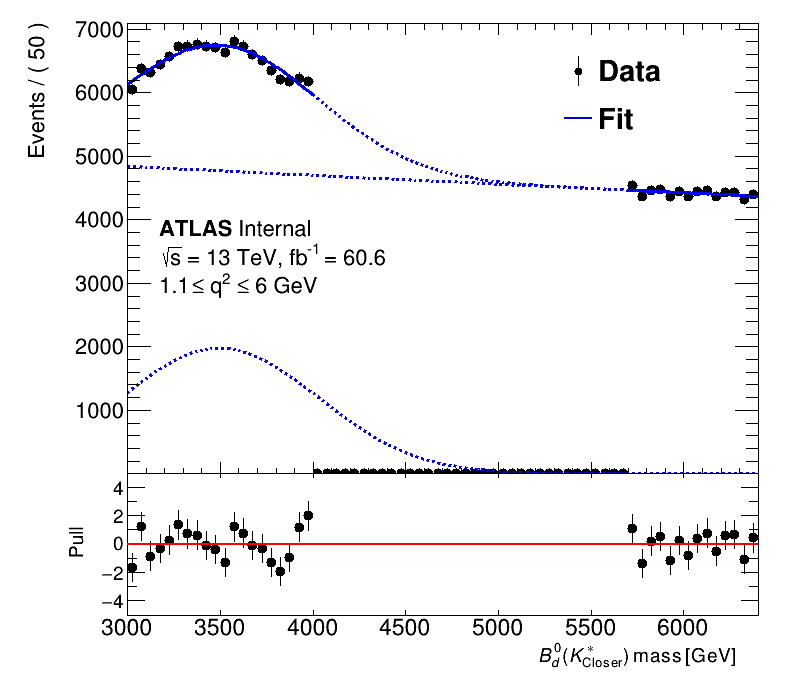
\includegraphics[width=0.5\textwidth]{figures/SidebandFit_CRSoptimisation.png}
    \caption{A blinded extended-likelihood fit to the invariant B mass in the low-$q^{2}$ signal region.
    Here the background shape is modelled by an exponential (combinatorial component) and a
    wide Gaussian (\lq B-like' background component). Below the pulls for the fit are also
    shown for the high-mass sideband.}
    \label{fig:SBFitCRS}
\end{figure}

To perform the 2D optimisation of the CRS, two CRS variables needed to be chosen.
These variables must have both good discriminating power between combinatorial
and \lq signal-like' decays and also exploit the information about the data.
To choose the first of the two variables, a significance scan was performed
on each of the CRS variables and the Punzi significance calculated at each
point in the scan (corresponding to varying the cut of each CRS variable).
In calculating the Punzi significance, the $\epsilon(t)$ was calculated as
the fraction of signal MC passing the cut, the value of $a$ was taken as 2,
and the background was calculated from a fit to the blinded low-$q^{2}$
sideband data. Here, assuming the sideband is a good approximation to the background,
we can calculate the number of background events $B(t)$ passing the cut
by rescaling our signal yield in the sidebands by the fraction of the blinded fit yield
in the signal region and sideband region. The blinded signal region of the low-$q^{2}$
data is defined as $m_{B} \in [4, 5.7]$\,GeV, whereas the sideband is defined
as the region $m_{B} \in [3.5, 4] \cup [5.7, 6.5]$\,GeV. Fig. \ref{fig:SBFitCRS}
shows the blinded fit to the low-$q^{2}$ invariant B mass distribution.
The signal-to-sideband ratio of the blinded fit yield is seen to be 0.567:0.433,
giving a normalisation factor of 1.31. The denominator in Eq.~\ref{eq:punzicalc}
can then be expressed as $1 + \sqrt{1.31B_{\textrm{SB}}(t)}$.
\begin{figure}[]
    \centering
    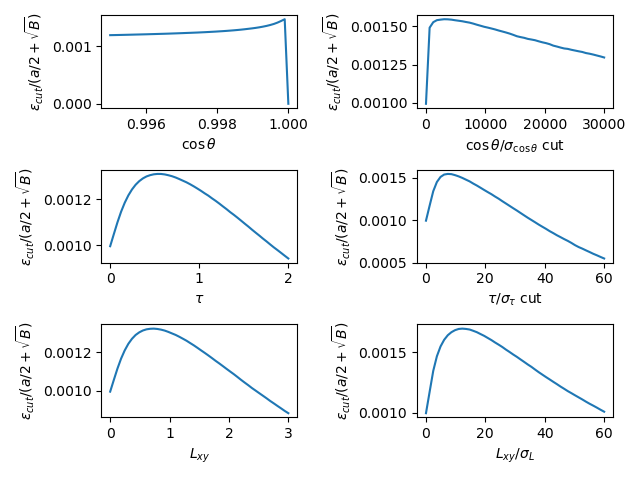
\includegraphics[width = 0.5\textwidth]{figures/PunziScan.png}
    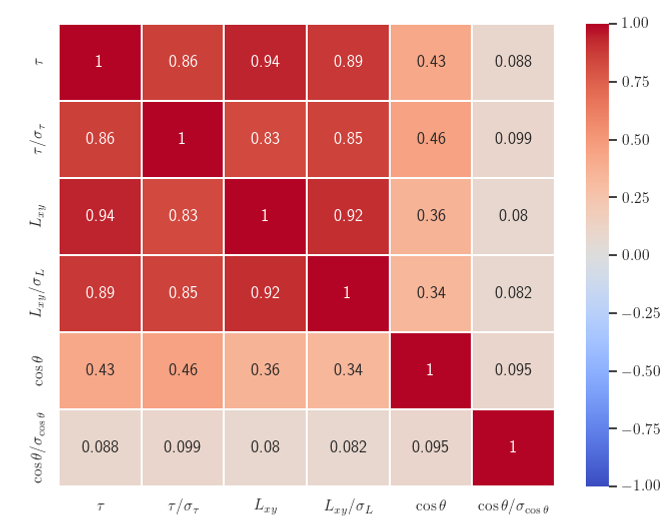
\includegraphics[width = 0.4\textwidth]{figures/CRSVarCorrs.png}
    \caption{Punzi significance scans for each of the 6 variables in the CRS optimisation,
    here the $L_{\textrm{xy}}$ significance value has the peak Punzi significance (left).
    The linear correlation coefficients between the various CRS variables (right).}
    \label{fig:PunziScans}
\end{figure}

For each of the Punzi significance scans, shown in Fig. \ref{fig:PunziScans}, the peak
significance was taken. These were then compared and the CRS variable with the highest
peak Punzi significance was chosen as the first variable for optimisation in the CRS.
This is seen to be the $L_{\textrm{xy}}$ significance. It is worth noting that
the Punzi significance does not correspond to a physically meaningful significance,
nor a sensitivity, instead, its maximum corresponds to a maximum sensitivity measurement,
i.e. by maximising the Punzi significance of our CRS scan we maximise our sensitivity
to the signal.

\begin{figure}
    \centering
    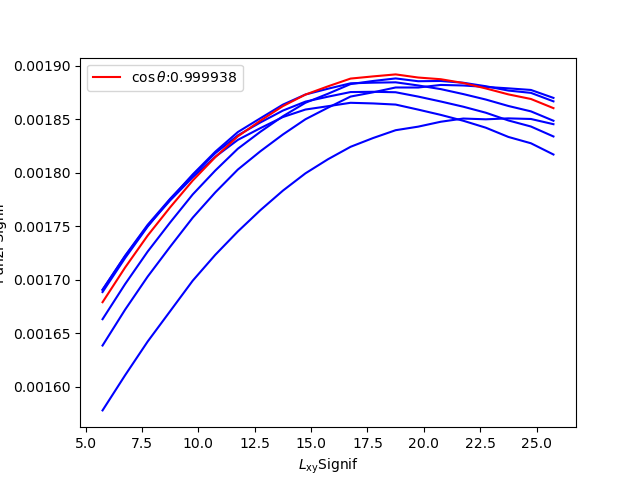
\includegraphics[width = 0.5\textwidth]{figures/2DPunziOpt.png}
    \caption{2D optimisation performed by scanning the Punzi significance of
    $\cos \theta$ significance cuts, for a given cut on the $L_{\textrm{xy}}$ significance.}
    \label{fig:2DCRSOpt}
\end{figure}

For choosing the second variable to be optimised, and with the idea of choosing the remaining
variable which would exploit the most information about the data, the correlations between
the CRS variables were calculated. These are shown in Fig \ref{fig:PunziScans}.
Having chosen the $L_{\textrm{xy}}$ significance as the first variable in the 2D CRS optimisation,
the second variable is the one with the smallest correlation coefficient with $L_{\textrm{xy}}$,
which is seen to be the $\cos \theta$ significance.
Finally, the 2D optimisation of the cuts in $(L_{\textrm{xy}}/\sigma_{L}, \cos \theta/\sigma_{\cos \theta})$
was done by performing a grid search maximisation of the Punzi significance for pairs of cuts.
Fig~\ref{fig:2DCRSOpt} shows the Punzi significance scan for a few slices of the grid search.
Optimum cuts on $(L_{\textrm{xy}}/\sigma_{L}, \cos \theta/\sigma_{\cos \theta})$ were found
to be $L_{\textrm{xy}}/\sigma_{L} >  15.8, \cos \theta/\sigma_{\cos \theta} > 0.016$.
\begin{figure}
    \centering
    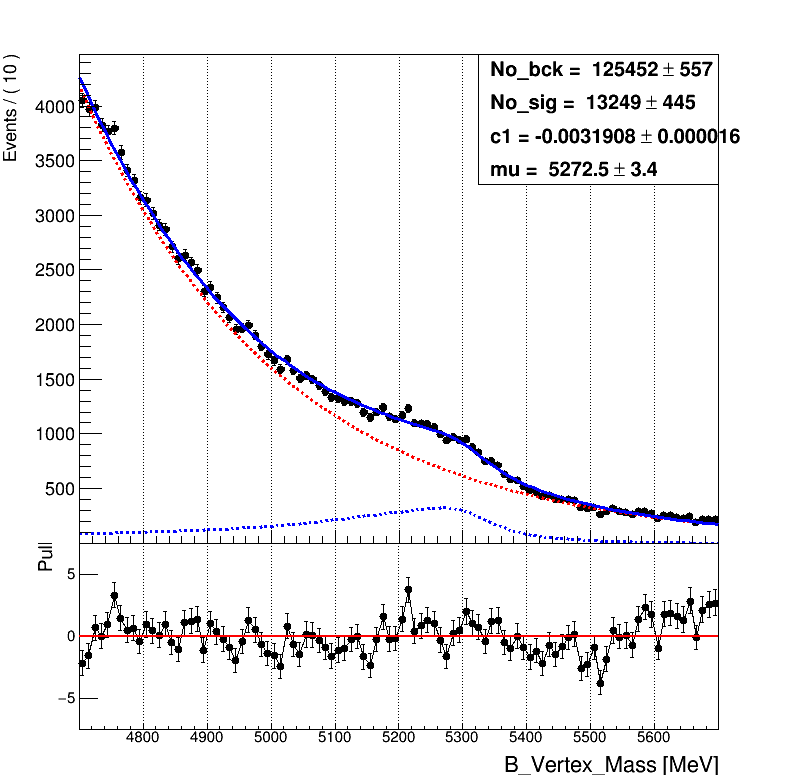
\includegraphics[width = 0.4\textwidth]{figures/B_masses_cutflow_JPsi_highq2_datafit.png}
    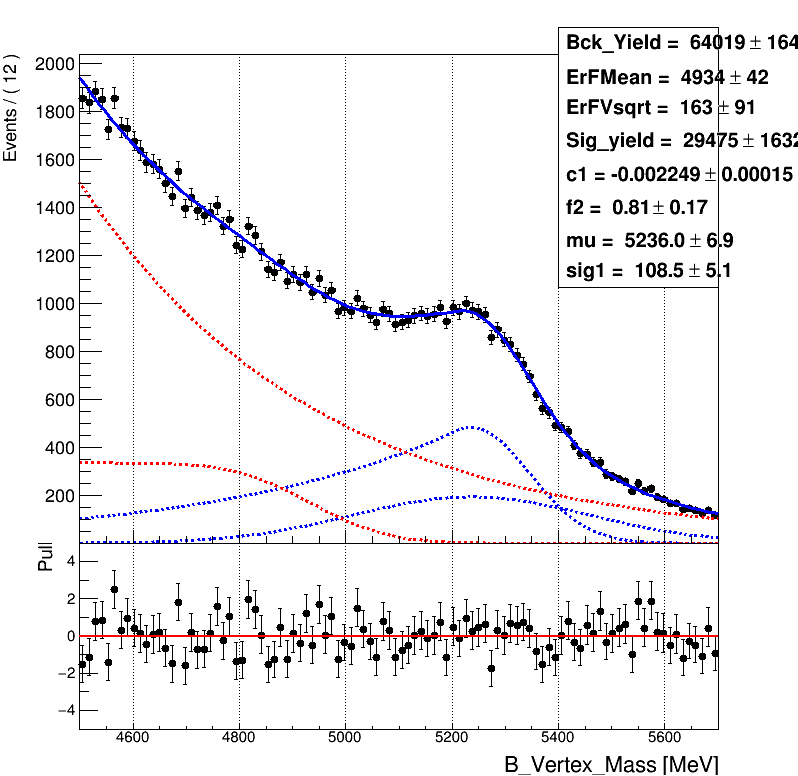
\includegraphics[width = 0.4\textwidth]{figures/BmassFit_Jpsi_Data_Highq2_CRS_extended_Bkgpdf_erfc_cores_free.png}
    \caption{(Left) Extended likelihood fits to the invariant B mass, with only the preselection applied,
    here signal is shown in blue and background in red. The fit results are also shown.
    (Right) Extended likelihood fits to the invariant B mass, with the preselection and
    additional CRS applied, here signal is shown in blue and background in red.
    The fit results are also shown. }
    \label{fig:CRSvsCutflowFits}
\end{figure}

The optimised CRS was then applied to the low-$q^{2}$ sideband data and also high-$q^{2}$ data
to assess the effect of the optimised selection on the reduction of combinatorial background.
For the high-$q^{2}$, this is particularly insightful as to the efficacy of the CRS,
as we see the emergence of the $J/\psi$ mass peak from the overwhelming background.
Fig.~\ref{fig:CRSvsCutflowFits} shows extended likelihood fits to the invariant B mass,
with and without the CRS applied. As can be seen, the CRS gives us a much better handle
on the functional form of the signal shape and allows us to safely factor
in the contribution of the \lq B-like' backgrounds in the background.


%-------------------------------------------------------------------------------
\section{Background Compositions}
\label{sec:background}
%-------------------------------------------------------------------------------
The backgrounds to the $B^0 \to K^*\ell^+\ell^-$ signal
are characterised by the following categories:

\begin{itemize}
\item combinatorial background, the dominant component due
  to uncorrelated tracks and characterised by a smooth descending
  shape in the $K\pi\ell\ell$ invariant mass;
\item resonant channel feed-down: this feeds into the low-mass sideband
  and it has a significantly high branching ratio;
\item misreconstructed or partially reconstructed decays, characterised by
  real $B$ decays to final states with similar enough compositions. Most of
  these decays have missing particles in the final states and thus accumulate
  in the low-mass sideband. A detailed study of the main contributions
  from these misreconstructed $B$ decays can be found below;
\item ``peaking'' background: $B^+ \to K^+\ell^+\ell^-$ or $B^+ \to J/\psi K^+$
  will contribute to the invariant mass distribution as a peaking structure
  on the right of the signal peak. (add decays with fakes here as well?)
\end{itemize}




\subsection{Discriminating Variables}
We describe here the discriminating variables used to separate
between the signal, the combinatorial background and the misreconstructed
$B$ decays.

The discriminating variables considered are the following:
\begin{itemize}
\item 
\end{itemize}


%-------------------------------------------------------------------------------
\section{Results}
\label{sec:result}
%-------------------------------------------------------------------------------

Place your results here.

% All figures and tables should appear before the summary and conclusion.
% The package placeins provides the macro \FloatBarrier to achieve this.
% \FloatBarrier

%-------------------------------------------------------------------------------
\section{Conclusion}
\label{sec:conclusion}
%-------------------------------------------------------------------------------

Place your conclusion here.

%-------------------------------------------------------------------------------
% If you use biblatex and either biber or bibtex to process the bibliography
% just say \printbibliography here.
\printbibliography
% If you want to use the traditional BibTeX you need to use the syntax below.
%\bibliographystyle{obsolete/bst/atlasBibStyleWithTitle}
%\bibliography{atlas-document,bib/ATLAS,bib/CMS,bib/ConfNotes,bib/PubNotes}
%-------------------------------------------------------------------------------

%-------------------------------------------------------------------------------
% Print the list of contributors to the analysis.
% The argument gives the fraction of the text width used for the names.
%-------------------------------------------------------------------------------
\clearpage
The supporting notes for the analysis should also contain a list of contributors.
This information should usually be included in \texttt{mydocument-metadata.tex}.
The list should be printed either here or before the Table of Contents.
\PrintAtlasContribute{0.30}

%-------------------------------------------------------------------------------
\clearpage
\appendix
\part*{Appendices}
\addcontentsline{toc}{part}{Appendices}
%-------------------------------------------------------------------------------

\section{Extra information on simulated and data samples}
\label{sec:app:data}
%-------------------------------------------------------------------------------
For completeness the correspondence between decay mode and Monte Carlo numbers
is given in Tables~\ref{tab:data:sig} and~~\ref{tab:data:bkg} for signal-like decays
and background channels, respectively.
\begin{table}[ht] 
\caption{Simulated samples for channels used as signal, reference and control decays.} 
\centering 
\rotatebox{90}{
\begin{tabular}{l l l l l l l l }
\hline\hline 
Run & decay & prod. & filter & pdg & XS * BR * & nEvents = & Sample Weight = XS * BR * \\ [0.5ex] 
number & process & xsec (nb) & eff. & (??) & * filter eff & sum weights & * genEff * lumi /nEvents  \\ [0.5ex] 
%heading 
\hline
Signal &  &  &  &  &  &  & \\
\hline
300578 & B+ -> K+ ee & 1.24E+05 & 9.15E-02 & 5.50E-07 & 6.23E-03 & 1497000 & 1.55E-01 \\
300579 & B- -> K- ee & 1.25E+05 & 9.10E-02 & 5.50E-07 & 6.24E-03 & 1497000 & 1.55E-01 \\
300580 & B+ -> K+ J/psi(ee) & 1.24E+05 & 8.60E-02 & 6.00E-05 & 6.39E-01 & "448 & 000" \\
300581 & B- -> K- J/psi(ee) & 1.25E+05 & 8.50E-02 & 6.00E-05 & 6.36E-01 & 447000 & 5.30E+01   \\
300582 & B+ -> K+ psi(2S) (ee) & 1.24E+05 & 9.98E-02 & 4.79E-06 & 5.91E-02 & 148000 & 1.49E+01 \\
300583 & B- -> K- psi(2S) (ee) & 1.24E+05 & 9.87E-02 & 4.79E-06 & 5.89E-02 & 150000 & 1.46E+01 \\
300590 & B0 -> K*0 ee & 1.24E+05 & 5.35E-02 & 6.59E-07 & 4.36E-03 & 1497500 & 1.08E-01 \\
300591 & B0bar -> anti-K*0 ee & 1.25E+05 & 5.29E-02 & 6.59E-07 & 4.34E-03 & 1497000 & 1.08E-01 \\
300592 & B0 -> K*0 J/psi(ee) & 1.24E+05 & 5.85E-02 & 5.02E-05 & 3.63E-01 & 447500 & 3.03E+01 \\
300593 & B0bar -> anti-K*0- J/psi(ee) & 1.25E+05 & 5.80E-02 & 5.02E-05 & 3.63E-01 & 449500 & 3.01E+01 \\
300594 & B0 -> K*0 psi(2S) (ee) & 1.24E+05 & 7.37E-02 & 3.03E-06 & 2.76E-02 & 150000 & 6.86E+00 \\
300595 & B0bar -> anti-K*0 psi(2S) (ee) & 1.25E+05 & 7.31E-02 & 3.03E-06 & 2.76E-02 & 150000 & 6.87E+00 \\
300706 & Bs -> phi ee & 2.74E+04 & 6.38E-02 & 4.01E-07 & 7.01E-04 & 1500000 & 1.74E-02 \\
300707 & Bsbar -> phi ee & 2.75E+04 & 6.39E-02 & 4.01E-07 & 7.06E-04 & 1497000 & 1.76E-02 \\
300708 & Bs -> phi J/psi(ee) & 2.74E+04 & 6.71E-02 & 3.14E-05 & 5.77E-02 & 450000 & 4.78E+00 \\
300709 & Bsbar -> phi J/psi(ee) & 2.75E+04 & 6.74E-02 & 3.14E-05 & 5.82E-02 & 450000 & 4.82E+00 \\
300710 & Bs ->phi psi(2S) (ee) & 2.74E+04 & 8.74E-02 & 2.04E-06 & 4.89E-03 & 150000 & 1.22E+00 \\
300711 & Bsbar -> phi psi(2S) (ee) & 2.75E+04 & 8.82E-02 & 2.04E-06 & 4.95E-03 & 150000 & 1.23E+00 \\ 
\hline
\end{tabular} 
}
\label{tab:data:sig}
\end{table}


\begin{table}[ht] 
\caption{Simulated samples for background decay channels.} 
\centering 
\rotatebox{90}{
\begin{tabular}{l l l l l l l l } 
\hline\hline
Run & decay & prod. & filter & pdg & XS * BR * & nEvents = & Sample Weight = XS * BR * \\ [0.5ex] 
number & process & xsec (nb) & eff. & (??) & * filter eff & sum weights & * genEff * lumi /nEvents  \\ [0.5ex] 
%heading 
\hline
Background samples &  &  &  &  &  &  & \\
\hline
300718 & B+ -> pi+ J/psi(ee) & 1.24E+05 & 8.87E-02 & 2.30E-06 & 2.53E-02 & 100000 & 9.44E+00 \\
300719 & B- -> pi- J/psi(ee) & 1.25E+05 & 8.78E-02 & 2.30E-06 & 2.52E-02 & 100000 & 9.38E+00 \\
300722 & B+ -> K+ pi0(eeg) & 1.24E+05 & 1.24E-02 & 1.51E-07 & 2.32E-04 & 99000 & 8.74E-02 \\
300723 & B- -> K- pi0(eeg) & 1.25E+05 & 1.22E-02 & 1.51E-07 & 2.29E-04 & 100000 & 8.53E-02 \\
300724 & B+ -> pi+ pi0(eeg) & 1.24E+05 & 1.28E-02 & 6.46E-08 & 1.02E-04 & 99000 & 3.86E-02 \\
300725 & B- -> pi- pi0(eeg) & 1.25E+05 & 1.25E-02 & 6.46E-08 & 1.01E-04 & 100000 & 3.75E-02 \\
300726 & B+ -> pi+ eta(eeg) & 1.24E+05 & 2.29E-02 & 2.81E-08 & 7.97E-05 & "99 & 000" \\
300727 & B- -> pi- eta(eeg) & 1.24E+05 & 2.24E-02 & 2.81E-08 & 7.84E-05 & 100000 & 2.92E-02 \\
300730 & B+ -> K+ eta(eeg) & 1.24E+05 & 2.21E-02 & 1.68E-08 & 4.58E-05 & 100000 & 1.71E-02 \\
300731 & B- -> K- eta(eeg) & 1.25E+05 & 2.18E-02 & 1.68E-08 & 4.56E-05 & 100000 & 1.70E-02 \\
300734 & B0 -> K+pi- J/psi(ee) & 1.24E+05 & 5.33E-02 & 6.83E-05 & 4.50E-01 & 100000 & 1.68E+02 \\
300735 & B0bar -> K-pi+ J/psi(ee) & 1.25E+05 & 5.27E-02 & 6.83E-05 & 4.48E-01 & 100000 & 1.67E+02 \\
300738 & B0 -> K+pi- psi(2S)(ee) & 1.24E+05 & 7.31E-02 & 4.48E-06 & 4.05E-02 & 98000 & 1.54E+01 \\
300739 & B0bar -> K-pi+ psi(2S)(ee) & 1.24E+05 & 7.28E-02 & 4.48E-06 & 4.06E-02 & 100000 & 1.51E+01 \\
300742 & B0 -> K+pi- pi0(eeg) & 1.24E+05 & 4.16E-03 & 4.44E-07 & 2.28E-04 & 100000 & 8.51E-02 \\
300743 & B0bar -> K-pi+ pi0(eeg) & 1.25E+05 & 4.01E-03 & 4.44E-07 & 2.22E-04 & 100000 & 8.27E-02 \\
300744 & B0 -> K*0 eta(eeg) & 1.24E+05 & 1.53E-02 & 7.41E-08 & 1.41E-04 & 100000 & 5.24E-02 \\
300745 & B0bar -> anti-K*0- eta(eeg) & 1.25E+05 & 1.51E-02 & 7.41E-08 & 1.40E-04 & 100000 & 5.21E-02 \\
300748 & B0 -> K*0 pi0(eeg) & 1.24E+05 & 8.82E-03 & 2.58E-08 & 2.82E-05 & 100000 & 1.05E-02 \\
300749 & B0bar -> anti-K*0- pi0(eeg) & 1.24E+05 & 8.65E-03 & 2.58E-08 & 2.78E-05 & 100000 & 1.04E-02 \\
\hline
\end{tabular} 
}
\label{tab:data:bkg}
\end{table}





\section{Extensive studies on backgrounds}
\label{sec:app:bkgdvij}
% This is both incomplete & not self-contained.
% The plots with better resolution are yet to be added.
% Relevant Indico: 
% - Real Backgrounds: https://indico.cern.ch/event/1200632/contributions/5048435/attachments/2513037/4319901/gnn-application-on-background-mc-samples.pdf
% - Fake Backgrounds: 
%    - More up-to-date: https://indico.cern.ch/event/1309827/contributions/5509564/attachments/2688607/4665119/fake-backgrounds-in-rkstar-updated.pdf
%    - More detailed: https://indico.cern.ch/event/1307390/contributions/5499421/attachments/2684051/4656482/background-for-RKStar-v2.pdf

% %%% Chapter Title %%%
% %%% ------------- %%%
% \chapter{A Study of ``Structured'' Backgrounds}
% \label{chap:a-study-in-fake}

%%% Introduction %%%
%%% ------------ %%%
\subsection{Introduction}
\label{subsec:back-intro}

Not all backgrounds are created equal; some are peskier than others. % 
In particular, any background that can form a \emph{distinctive structure} in its distribution in the discriminating variable, i.e., the variable in whose distribution the final fit is performed, needs to be studied in its own right. %
\\\\
As such, we expect the most dominant sources of background to be combinatorial and partially reconstructed decays. %
Such sources of background are not expected to form any distinctive structure in their distribution of $m(B)$ which is the discriminating variable in this analysis. %   
Outside of the combinatorial and the partially reconstructed sources of background, which are essentially monotonic (i.e. non-structured), there exist other sources of background that can be genuinely distinctively structured in the signal region of $m(B)$. %
One can identify two such sources of background:
\begin{enumerate}
    \item \textbf{Real Backgrounds}: The decays of particles whose masses lie in the fit-region of $m(B)$ and whose decay structures (number of final-state particles, their vertexing, etc.) are similar to that of the signal decay. 
    \item \textbf{Fake Backgrounds}: The decays of particles whose masses lie in the fit-region of $m(B)$ and whose decay structures can be made to look similar to that of the signal decay if the final-state particles are misidentified.
\end{enumerate} 
One important point to notice is that despite such sources of backgrounds being significantly subdominant compared to the combinatorial and partially reconstructed decays, they matter just as much (in terms of the analysis strategy) so long as their yield is comparable to the signal yield, as it was well demonstrated in the LHCb measurement from December 2022~\cite{LHCbDec2022}. % 
Given that we are measuring a rare decay with a branching fraction $\mathcal{O}(10^{-6})$, we are precisely in the situation, where we cannot neglect even such subdominant sources of background. % 
\\\\
Our goal in the study of these backgrounds is to understand two aspects:
\begin{enumerate}
    \item Do they actually form a distinctive (non-monotonic) structure in the distribution of $m(B)$? 
    \item If they do, how do we deal with them?
    \begin{itemize}
        \item Can some targeted cuts be applied to reject them?
        \item If not, how should these be modeled in the final fit?
    \end{itemize}
\end{enumerate}
The study of such backgrounds with the goals outlined above constitutes the majority of the ongoing work in the analysis. %
In the following, I will outline the strategy that we are following to study such backgrounds.

%%% The Real Backgrounds %%%
%%% -------------------- %%%
\subsection{The Real Backgrounds}
\label{subsec:the-real-backgrounds}

The real backgrounds in this analysis are expected to arise from the decays of $B$-hadrons other than the signal decay. %
Since such decays are expected to look very similar to signal decay, we cannot easily reject them using either heuristic cuts or multivariate techniques without losing much of our signal efficiency. % 
However, specific sources of real backgrounds can be targeted by designing specific heuristic cuts, for example, $B_s^0 \to \phi(1020)(\to K^+K^-) \ell^+\ell^-$ can be targeted by rejecting events with an invariant mass of the $K^+K^-$ pair that is very close to the $\phi(1020)$ meson (this cut is already employed). %
The residual of the real backgrounds needs to be modeled in the final fit (for example, as in the $B^+$ case discussed earlier). %
We are working on both the design of the cuts to reject specific sources of real backgrounds as well as the modeling of the residual of the real backgrounds in the final fit. %
These backgrounds are expected to form a peaking structure under the signal $B-$mass, particularly in the high$-q^2$ bin as can be seen in Fig.~\ref{fig:peaking-real-background-mc}. %
Both of these efforts rely on the use of the MC simulation of the relevant backgrounds. %
In particular, the shape of the fit model of the residual of the real backgrounds is to be obtained from the MC simulation of the relevant backgrounds while the yield of the residual of the real backgrounds is to be tied to the yield of the signal in the resonant channel. %
\begin{figure}[!ht]
    \centering
    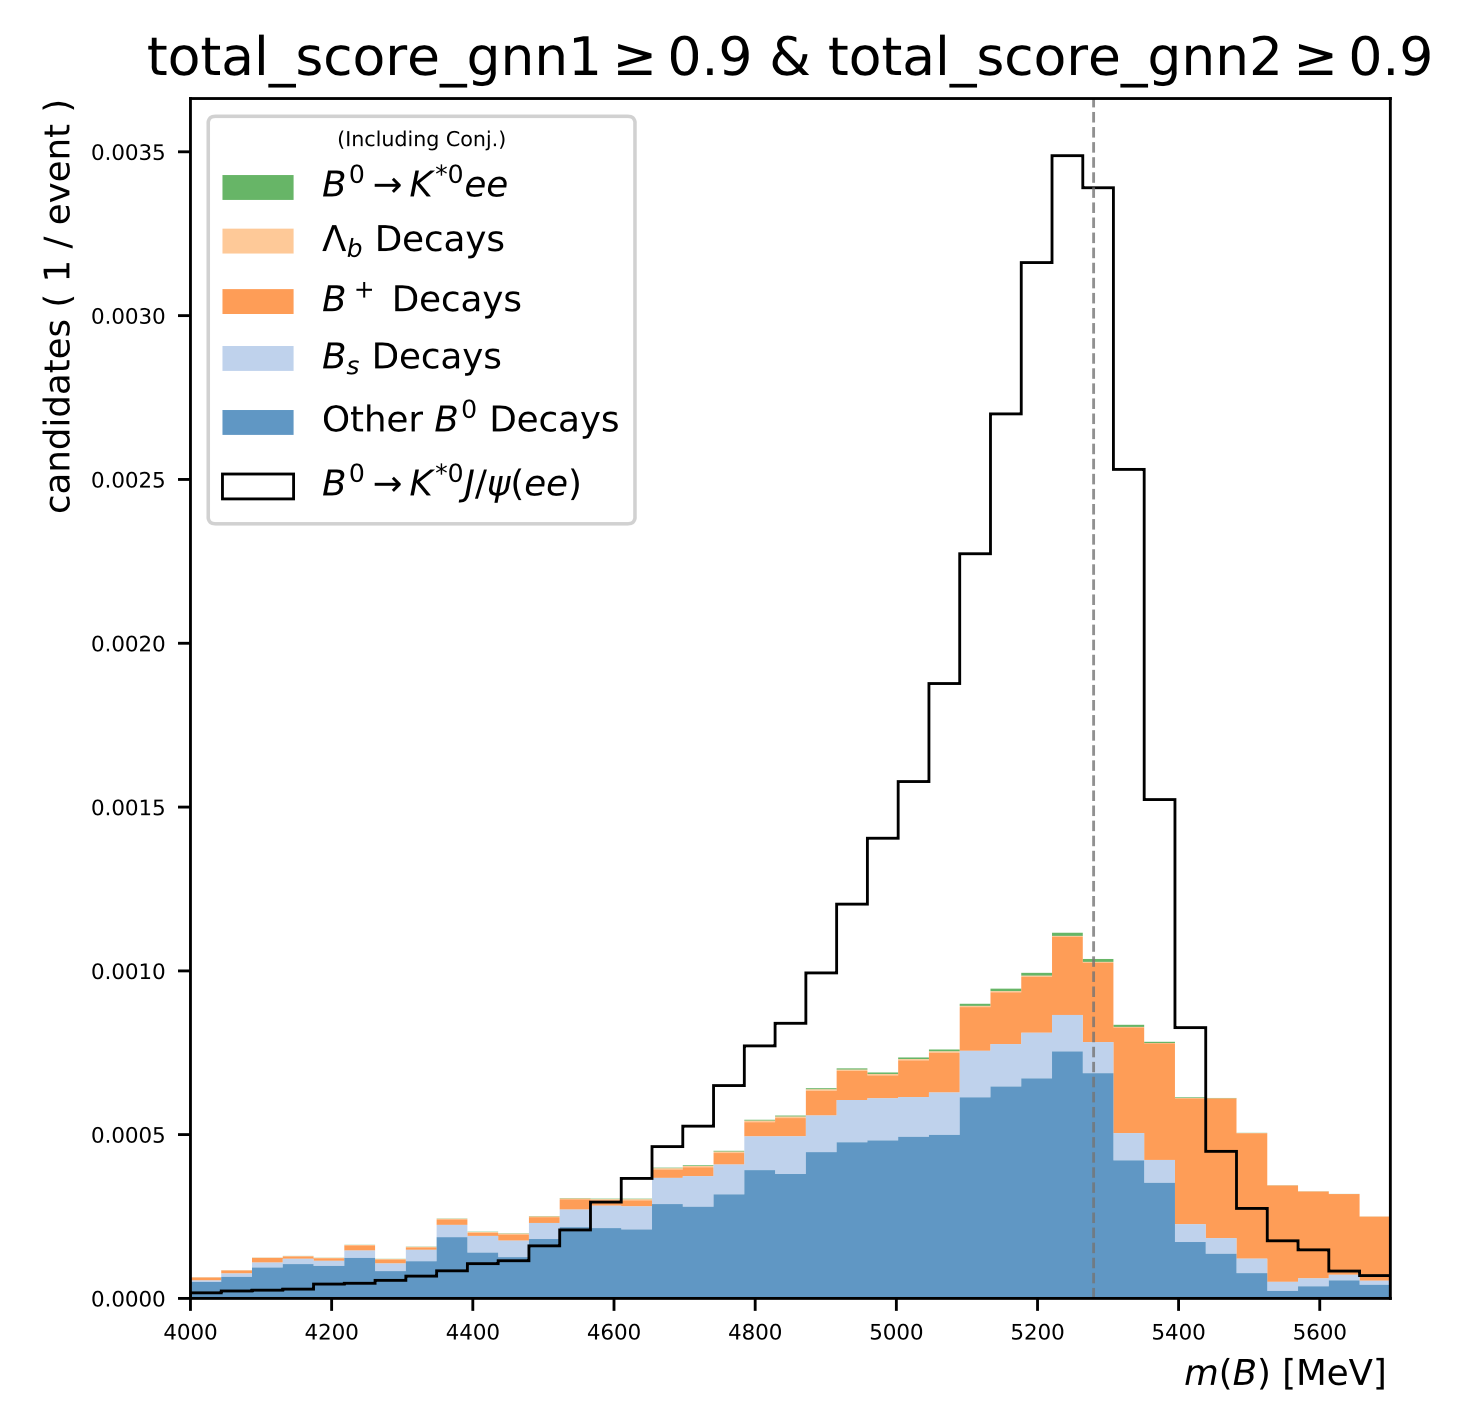
\includegraphics[width=0.48\textwidth]{figures/stacked-b-mass-q2high.png}
    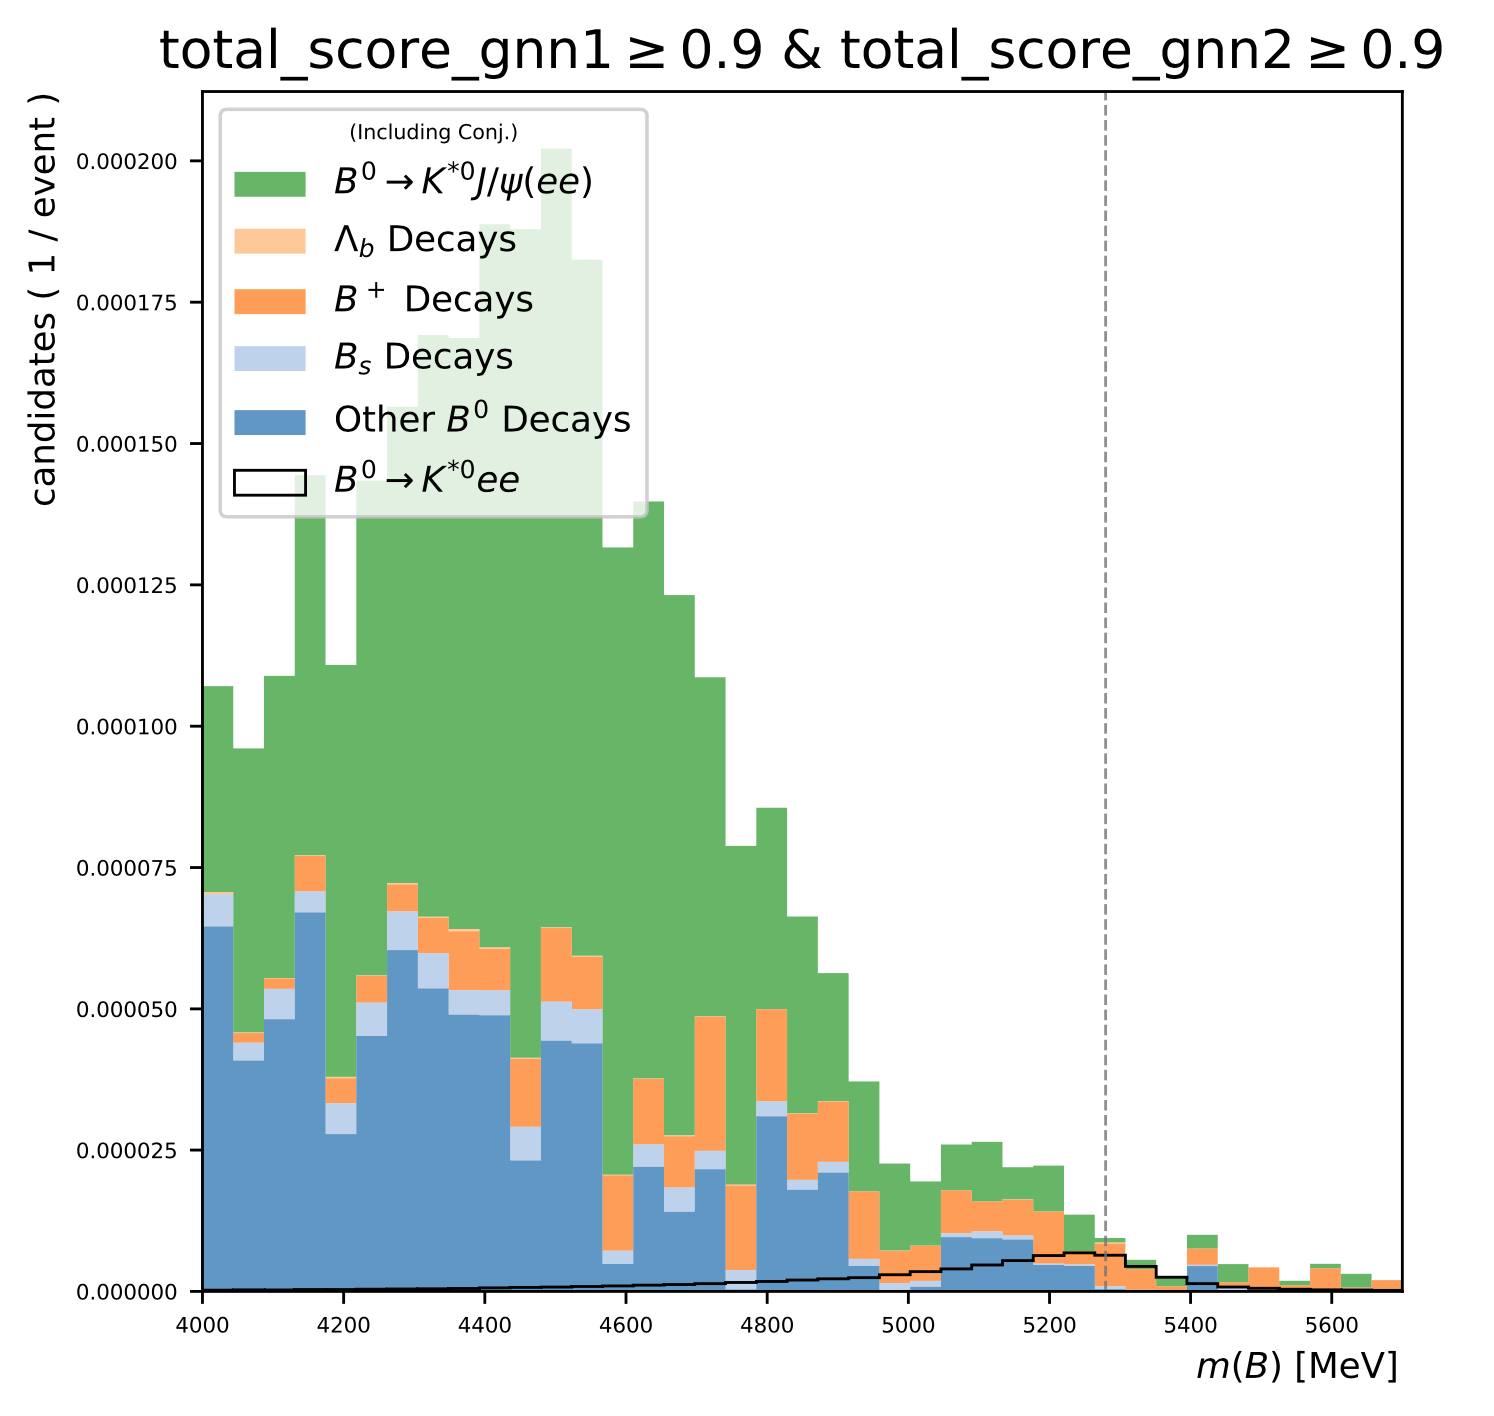
\includegraphics[width=0.48\textwidth]{figures/stacked-b-mass-q2low.png}
    \caption{Comparison of the signal to the cumulative contribution from major sources of real background after stringent cuts on the GNN scores: signal being $B_d^0\to K^{\ast 0}(K^+\pi^-)J/\psi(e^+e^-)$ in the high$-q^2$ bin (left), $B_d^0\to K^{\ast 0}(K^+\pi^-)e^+e^-$ in the low$-q^2$ bin (right). All distributions are normalized to the same (albeit arbitrary) luminosity so as to correctly represent their relative yields.}
    \label{fig:peaking-real-background-mc}
\end{figure}
\\\\
We are currently running a large MC campaign to complete the list of real backgrounds for completeness where the list is being compiled using the~{\texttt{decaylanguage}} package\footnote{\href{https://github.com/scikit-hep/decaylanguage}{\texttt{\textcolor{olive}{https://github.com/scikit-hep/decaylanguage}}}}. %
This is relevant for both the electron and the muon channels of the measurement. %

%%% The Fake Backgrounds %%%
%%% -------------------- %%%
\subsection{The Fake Backgrounds}
\label{subsec:the-fake-backgrounds}

The $R(X)$ measurement is particularly sensitive to the estimation of the fake backgrounds in the electron channel. %
For example, as mentioned earlier, the source of tension with the SM in the pre-2022 LHCb measurements of $R(K)$ and $R(K^{\ast})$ has been attributed to the missing estimation of the background arising from hadrons faking electrons. % 
Also in this analysis, the fake backgrounds are expected to arise from the misidentification of final-state hadrons (mostly pions, kaons, and protons) as electrons or muons; as well as, to a lesser extent, from the misidentification of final-state photons as electrons via the conversion of the photon into an $e^+e^-$ pair in the detector material. %
\\\\
We are studying three different methods to model the fake backgrounds in the final fit: the matrix method, the reverse-region method, and the MC-driven method. % 
The first two of these methods are data-driven methods while the third one simply relies on the MC simulation of the relevant backgrounds. %
It is usually considered unreliable to purely rely on the MC simulation of the fake backgrounds because the MC simulation is not expected to model the misidentification rates very well. %
However, the MC-driven method is still useful as a cross-check on the other two methods. %
Concerning the data-driven method, the bottleneck is the availability of a fake-enriched region of the data. %
This is a control region of the data, where we expect the hadrons to be the dominant source of reconstructed leptons. %
\\\\
In the electron channel, the methods that are traditionally used to define such a region are not applicable: we cannot use the isolation variables to define the fake-enriched region because both the signal and the fake backgrounds are expected to be non-isolated; we cannot easily reverse the particle identification cuts because our electrons are already at the loosest possible working point of the particle identification. %
Thus, we are exploring the utilization of low-level information associated with the tracks of the reconstructed leptons to define a fake-enriched region of the data. %
Another ongoing effort is the study of decay modes that are expected to be particularly important in the estimation of fake backgrounds. %
It is crucial to prepare a representative sample of the fake backgrounds in the MC simulation. %
Such a sample is also necessary to validate the extraction of the fake-enriched region in the data-driven methods. %
We are currently running a large MC campaign to complete the list of fake backgrounds where the list is being compiled using the~{\texttt{decaylanguage}} package mentioned earlier. %
This is relevant mainly for the electron channel of the measurement. %
\\\\
The estimation of the fake muon background will follow with more traditional methods since the muons are not at the loosest identification levels. %
In addition, the impact of fake muons is usually much smaller compared to the one from fake electrons. %
\\\\


\end{document}
